\documentclass[a4paper,oneside,12pt]{report}
% Package yang diperlukan
\usepackage{graphicx}      % Untuk memasukkan gambar
\usepackage{titling}       % Untuk kustomisasi halaman judul
\usepackage{geometry}      % Untuk mengatur margin halaman
\usepackage{listings}      % Untuk menampilkan blok kode
\usepackage{xcolor}        % Untuk menggunakan warna
\usepackage{float}         % Untuk kontrol penempatan float (seperti gambar)
\usepackage{hyperref}      % Untuk membuat hyperlink (URL, referensi)
\usepackage{indentfirst}   % Untuk memberi indentasi pada paragraf pertama setiap seksi
\usepackage{url}           % Untuk format URL
\usepackage{fancyhdr}      % Untuk kustomisasi header dan footer
\usepackage{tocloft}       % Untuk kustomisasi Daftar Isi
\usepackage{bookmark}      % Untuk manajemen bookmark PDF yang lebih baik

%======================================================================
% PENGATURAN GEOMETRI HALAMAN
%======================================================================
% Margin umum untuk isi laporan
\geometry{left=3cm, right=2.5cm, top=2cm, bottom=2.5cm}
\sloppy

%======================================================================
% PENGATURAN WARNA UNTUK BLOK KODE
%======================================================================
\definecolor{codegreen}{rgb}{0,0.6,0}
\definecolor{codegray}{rgb}{0.5,0.5,0.5}
\definecolor{codepurple}{rgb}{0.58,0,0.82}
\definecolor{backcolour}{rgb}{0.95,0.95,0.92}
\definecolor{darkblue}{rgb}{0,0,0.6}

%======================================================================
% PENGATURAN BLOK KODE (LISTINGS)
%======================================================================
% Gaya umum untuk semua blok kode
\lstdefinestyle{commonstyle}{
    backgroundcolor=\color{backcolour}, 
    breakatwhitespace=false, 
    breaklines=true, 
    captionpos=b, 
    keepspaces=true,
    numbers=left, 
    numbersep=5pt, 
    showspaces=false, 
    showstringspaces=false,
    showtabs=false, 
    tabsize=2, 
    frame=single,
    basicstyle=\ttfamily\footnotesize,
    numberstyle=\tiny\color{codegray},
    columns=flexible,
    postbreak=\mbox{\textcolor{red}{$\hookrightarrow$}\space},
    breakindent=0pt,
    breakautoindent=false
}

% Gaya khusus untuk HTML
\lstdefinestyle{htmlstyle}{
    style=commonstyle,
    language=HTML,
    commentstyle=\color{codegreen},
    keywordstyle=\color{codepurple},
    stringstyle=\color{codegreen},
    basicstyle=\ttfamily\scriptsize
}

% Gaya khusus untuk CSS
\lstdefinestyle{cssstyle}{
    style=commonstyle,
    commentstyle=\color{codegreen},
    keywordstyle=\color{darkblue},
    stringstyle=\color{codepurple},
    emph={color, background, font, margin, padding, border, display, position, width, height},
    emphstyle=\color{darkblue},
    basicstyle=\ttfamily\scriptsize
}

% Gaya khusus untuk Python
\lstdefinestyle{pythonstyle}{
    style=commonstyle,
    language=Python,
    commentstyle=\color{codegreen},
    keywordstyle=\color{darkblue},
    stringstyle=\color{codepurple},
    emph={import,from,class,def,for,while,if,else,elif,try,except,finally},
    emphstyle=\color{darkblue}
}

% Gaya khusus untuk SQL
\lstdefinestyle{sqlstyle}{
    style=commonstyle,
    language=SQL,
    commentstyle=\color{codegreen},
    keywordstyle=\color{darkblue},
    stringstyle=\color{codepurple},
    emph={SELECT,FROM,WHERE,INSERT,UPDATE,DELETE,CREATE,DROP},
    emphstyle=\color{darkblue}
}

% Gaya khusus untuk JavaScript/JSON
\lstdefinestyle{javascriptstyle}{
    style=commonstyle,
    commentstyle=\color{codegreen},
    keywordstyle=\color{darkblue},
    stringstyle=\color{codegreen},
    emph={function,var,let,const,return,if,for,while,do,else,switch,case,jwt,message,expireAt,first_name,last_name,email,password,role},
    emphstyle=\color{darkblue}
}

% Gaya khusus untuk PHP
\lstdefinestyle{phpstyle}{
    style=commonstyle,
    language=PHP,
    commentstyle=\color{codegreen},
    keywordstyle=\color{darkblue},
    stringstyle=\color{codepurple},
    emph={php,include,require,return,new,public,function,class,extends,try,catch},
    emphstyle=\color{darkblue}
}

%======================================================================
% PENGATURAN LAIN-LAIN
%======================================================================
% Perintah kustom untuk bingkai gambar
\newcommand{\customfbox}[1]{%
  \setlength{\fboxsep}{0pt}%
  \setlength{\fboxrule}{0.5pt}%
  \fcolorbox{black}{white}{#1}%
}

% Mengganti nama default "Figure" menjadi "Gambar"
\renewcommand{\figurename}{Gambar}
\renewcommand{\thefigure}{\arabic{figure}}

% Pengaturan Hyperlink
\hypersetup{
    colorlinks=true, 
    linkcolor=black, 
    filecolor=black, 
    urlcolor=black,
    citecolor=black,
    pdftitle={Laporan Praktikum Pertemuan XI}, 
    pdfpagemode=FullScreen, 
    breaklinks=true
}

% Pengaturan Header & Footer (nomor halaman di tengah bawah)
\pagestyle{fancy}
\fancyhf{}
\fancyfoot[C]{\thepage}
\renewcommand{\headrulewidth}{0pt}

\fancypagestyle{plain}{
    \fancyhf{}
    \fancyfoot[C]{\thepage}
    \renewcommand{\headrulewidth}{0pt}
}

%======================================================================
% PENGATURAN STRUKTUR BAB DAN DAFTAR ISI
%======================================================================
\renewcommand{\contentsname}{Daftar Isi}
\renewcommand{\bibname}{Daftar Pustaka}

% Menghilangkan nomor bab tetapi mempertahankan penomoran seksi
\renewcommand{\thechapter}{}
\renewcommand{\chaptername}{}

% Format penomoran seksi menjadi [nomor bab].[nomor seksi]
\renewcommand{\thesection}{\arabic{chapter}.\arabic{section}}
\renewcommand{\thesubsection}{\thesection.\arabic{subsection}}

\setcounter{secnumdepth}{3}
\setcounter{tocdepth}{3}

% Format Daftar Isi (TOC)
\renewcommand{\cftchapdotsep}{\cftdotsep}
\renewcommand{\cftchapleader}{\cftdotfill{\cftchapdotsep}}
\setlength{\cftchapindent}{0em}
\setlength{\cftsecindent}{2em}
\setlength{\cftsubsecindent}{4em}
\setlength{\cftchapnumwidth}{0em}
\setlength{\cftsecnumwidth}{2.5em}
\setlength{\cftsubsecnumwidth}{3.2em}
\renewcommand{\cftchappresnum}{}
\renewcommand{\cftchapaftersnum}{}

% Perintah kustom untuk membuat judul bab di TOC menjadi tebal
\newcommand{\tocboldsection}[1]{%
  \protect\renewcommand{\protect\cftchapfont}{\protect\bfseries}%
  #1%
  \protect\renewcommand{\protect\cftchapfont}{}%
}

%======================================================================
% AWAL DOKUMEN
%======================================================================
\begin{document}

% Halaman Judul
\newgeometry{left=3cm, right=2.5cm, top=2cm, bottom=2cm}
\begin{titlingpage}
\begin{center}
\vspace*{0.3cm}
{\large \textbf{\MakeUppercase{Laporan Praktikum}}} \\[0.3cm]
{\large \textbf{\MakeUppercase{SISTEM ADMINISTRASI DAN INFORMASI TERDISTRIBUSI}}} \\[0.3cm]
{\large \textbf{\MakeUppercase{Pertemuan XI}}} \\[0.3cm]
{\large \textbf{\MakeUppercase{ORKESTRASI DOCKER DENGAN DOCKER COMPOSE}}} \\[0.8cm]


\includegraphics[height=7cm]{lambang ugm.png} \\[0.8cm]

{\normalsize \textbf{Disusun oleh:}} \\[0.3cm]
\begin{tabular}{@{}l l @{}}
  \textbf{Nama}             & : Januarsyah Akbar \\
  \textbf{NIM}              & : 24/535846/SV/24314 \\
  \textbf{Kelas}            & : B2 \\
  \textbf{Dosen Pengampu}   & : Dr. Imam Fahrurrozi, S.T., M.Cs.
\end{tabular} \\[1.5cm]

{\normalsize \textbf{PROGRAM STUDI D-IV}} \\[0.15cm]
{\normalsize \textbf{TEKNOLOGI REKAYASA PERANGKAT LUNAK}} \\[0.15cm]
{\normalsize \textbf{DEPARTEMEN TEKNIK ELEKTRO DAN INFORMATIKA}} \\[0.15cm]
{\normalsize \textbf{SEKOLAH VOKASI}} \\[0.15cm]
{\normalsize \textbf{UNIVERSITAS GADJAH MADA}} \\[0.15cm]
{\normalsize \textbf{YOGYAKARTA}} \\[0.15cm]
{\normalsize \textbf{2026}}
\end{center}
\end{titlingpage}
\restoregeometry

% Halaman kosong setelah cover (halaman i, tidak bernomor)
\clearpage
\pagenumbering{roman}
\setcounter{page}{1}
\thispagestyle{empty}

% --- Daftar Isi (halaman ii) ---
\clearpage
\setcounter{page}{2}
\addcontentsline{toc}{chapter}{Daftar Isi}
\tableofcontents
\clearpage

% Mengatur penomoran halaman menjadi arab dan mulai dari 1
\pagenumbering{arabic}
\setcounter{page}{1}

\chapter[Tujuan Praktikum]{Tujuan Praktikum}
\begin{enumerate}
    \item Memahami perbedaan antara \textit{Dockerfile} (membangun \textit{image}) dan \textit{Docker Compose} (menjalankan \textit{container}).
    \item Mentranslasikan perintah CLI \texttt{docker run} yang panjang menjadi file konfigurasi \texttt{docker-compose.yml}.
    \item Mengimplementasikan fitur \textit{Volumes} untuk \textit{Hot-Reloading} (perubahan kode langsung terlihat tanpa \textit{rebuild}).
    \item Mengelola \textit{environment variables} menggunakan \texttt{.env} yang terintegrasi dengan \textit{Docker Compose}.
\end{enumerate}
\clearpage

\chapter{Dasar Teori}

\section{Docker Compose}
Sebelumnya kita telah belajar mengenai \textit{Dockerfile}. Mempelajari \textit{Dockerfile} dalam waktu singkat sungguh melelahkan dan penuh tantangan. Di pertemuan kali ini, kita akan mempelajari \textit{Docker Compose}, yang tentunya akan terasa lebih mudah. Jika \textit{Dockerfile} adalah ``Resep Makanan'' (cara membuat \textit{Image}), maka \textit{Docker Compose} adalah ``Daftar Menu \& Pelayan'' yang mengatur bagaimana hidangan tersebut disajikan di meja makan (\textit{Container}).

\textit{Docker Compose} adalah alat (\textit{tool}) untuk mendefinisikan dan menjalankan aplikasi Docker multi-kontainer (walaupun bisa juga untuk satu kontainer). Dengan \textit{Docker Compose}, kita menggunakan file YAML untuk mengonfigurasi layanan aplikasi, jaringan, dan volume. File YAML \textit{Docker Compose} memiliki beberapa bagian penting, di antaranya \textit{Version}, \textit{Services}, \textit{Volume}, dan \textit{Networks} \cite{docker_docs}.

Beberapa komponen utama dalam konfigurasi \textit{Docker Compose} meliputi:
\begin{itemize}
    \item \textbf{Services}: Merupakan daftar kontainer (\textit{container}) yang akan dijalankan, seperti \textit{app-server}, \textit{database}, dan lain-lain sesuai dengan kebutuhan sistem.
    \item \textbf{Volumes}: Merupakan pemetaan (\textit{mapping}) folder dari \textit{host} ke kontainer agar data dapat tersimpan secara permanen atau untuk mempercepat proses pengembangan (\textit{development}) seperti fitur \textit{hot-reload}.
    \item \textbf{Networks}: Merupakan jaringan virtual terisolasi yang menghubungkan antar-\textit{services} agar dapat saling berkomunikasi secara aman melalui resolusi nama layanan internal.
\end{itemize}

\section{Perbedaan Dockerfile dan Docker Compose}
Meskipun keduanya digunakan dalam ekosistem Docker, peran masing-masing sangat berbeda secara mendasar:
\begin{itemize}
    \item \textbf{Dockerfile}: Adalah deskripsi atau instruksi pembuatan \textit{blueprint} tunggal (\textit{Image}) untuk satu aplikasi spesifik (misalnya menentukan OS dasar, menginstal dependensi perangkat lunak, dan menyalin kode sumber).
    \item \textbf{Docker Compose}: Berfungsi sebagai pengorkestrasi banyak kontainer sekaligus agar dapat berjalan selaras, mendefinisikan interkoneksi, pemetaan port fisik, dan ketergantungan antar-kontainer tanpa harus menuliskan argumen CLI yang panjang di terminal.
\end{itemize}

\section{Perintah Dasar Docker Compose}
\textit{Docker Compose} memiliki perintah-perintah (\textit{commands}) utama yang serupa dengan Docker, di antaranya:
\begin{itemize}
    \item \texttt{docker compose up}: Digunakan untuk membangun, membuat, dan menjalankan kontainer.
    \item \texttt{docker compose down}: Digunakan untuk menghentikan dan menghapus kontainer serta jaringan (\textit{network}) virtual.
    \item \texttt{docker compose logs -f}: Digunakan untuk melihat \textit{log output} dari seluruh layanan (\textit{services}) secara real-time.
\end{itemize}

\section{Volumes dan Mekanisme Hot-Reload}
Secara default, kontainer Docker bersifat \textit{stateless} and \textit{ephemeral} (data di dalamnya akan hilang saat kontainer dihapus). Volume hadir untuk memecahkan masalah ini dengan dua jenis metode:
\begin{itemize}
    \item \textbf{Volume Binding (Bind Mounts)}: Memetakan folder proyek lokal langsung ke direktori kontainer (misalnya \texttt{.:/var/www/html}). Fitur ini sangat krusial selama pengembangan karena memungkinkan fitur \textbf{Hot-Reloading}, yaitu perubahan kode lokal langsung tercermin di dalam kontainer secara instan tanpa perlu rebuild image.
    \item \textbf{Persistent Volumes}: Folder volume khusus yang dikelola oleh sistem Docker host untuk menjamin data (seperti file database MySQL) tetap tersimpan aman dan tidak hilang meskipun kontainer di-restart atau dihapus.
\end{itemize}

\clearpage

\chapter[\texorpdfstring{\tocboldsection{Hasil dan Pembahasan}}{Hasil dan Pembahasan}]{Hasil dan Pembahasan}

\section{Sinkronisasi dan Persiapan Proyek}

\subsection{Kloning dan Sinkronisasi Berkas}
Langkah awal pengerjaan dimulai dengan mengkloning repositori boilerplate mentah \texttt{php-jwt-example} menggunakan Git:
\begin{lstlisting}[style=commonstyle, language=bash]
git clone https://github.com/hananhanafi/php-jwt-example.git
\end{lstlisting}
Karena repositori yang dicloning masih berupa codebase awal, kami menyalin berkas-berkas hasil pengembangan kontainerisasi dari pertemuan sebelumnya (seperti \texttt{Dockerfile}, \texttt{.htaccess}, \texttt{.env}, \texttt{index.php} router, dan \texttt{config/database.php}) ke root direktori proyek agar fungsionalitas dasar aplikasi telah siap pakai.

\subsection{Koreksi Path Impor Absolut}
Untuk mengeliminasi error pemanggilan berkas PHP akibat ketidaksesuaian root pemanggilan pada saat dijalankan melalui router pusat (\texttt{index.php}) maupun secara mandiri, kami memodifikasi file sub-endpoint pada folder \texttt{api/} dengan menyematkan konstanta \texttt{\_\_DIR\_\_}.

- \textbf{File \texttt{api/register/index.php}}:
\begin{lstlisting}[style=phpstyle]
include_once __DIR__ . '/../../config/database.php';
\end{lstlisting}

- \textbf{File \texttt{api/login/index.php} dan \texttt{api/users/index.php}}:
\begin{lstlisting}[style=phpstyle]
include_once __DIR__ . '/../../config/database.php';
require __DIR__ . "/../../vendor/autoload.php";
\end{lstlisting}

\section{Konfigurasi Docker Compose Terintegrasi}
Kami membuat berkas baru bernama \texttt{docker-compose.yml} pada direktori root proyek untuk mengorkestrasikan tiga layanan utama (\texttt{be-jwt}, \texttt{database\_mysql}, dan \texttt{phpmyadmin}) dalam satu arsitektur jaringan virtual \texttt{psait}.

\begin{lstlisting}[style=commonstyle]
services:
  # Service Backend PHP-Apache
  be-jwt:
    container_name: php-jwt-example
    build: .
    ports:
      - "8080:8080" # Apache berjalan pada port 8080 di Dockerfile
    volumes:
      - .:/var/www/html # Bind mount untuk fitur Hot Reload
    env_file:
      - .env
    restart: unless-stopped
    networks:
      - psait
    depends_on:
      - database_mysql

  # Service Database MySQL
  database_mysql:
    image: mysql:8.0
    container_name: db_mysql_jwt
    restart: unless-stopped
    networks:
      - psait
    volumes:
      - db_data:/var/lib/mysql
      - ./php_jwt_db.sql:/docker-entrypoint-initdb.d/init.sql # Inisialisasi basis data
    environment:
      MYSQL_DATABASE: ${DB_NAME}
      MYSQL_USER: ${DB_USER}
      MYSQL_PASSWORD: ${DB_PASSWORD}
      MYSQL_ALLOW_EMPTY_PASSWORD: "yes"
      MYSQL_ROOT_PASSWORD: ${DB_ROOT_PASS:-""}

  # Service phpMyAdmin (TUGAS)
  phpmyadmin:
    image: phpmyadmin:latest
    container_name: phpmyadmin_jwt
    restart: unless-stopped
    ports:
      - "8081:80" # Akses phpMyAdmin via host port 8081
    networks:
      - psait
    environment:
      PMA_HOST: database_mysql
      PMA_PORT: 3306
      PMA_USER: ${DB_USER}
      PMA_PASSWORD: ${DB_PASSWORD}
      MYSQL_ROOT_PASSWORD: ${DB_ROOT_PASS:-""}
    depends_on:
      - database_mysql

# Definisi Jaringan Virtual bersama
networks:
  psait:
    driver: bridge

# Definisi Volume Persisten untuk MySQL
volumes:
  db_data:
\end{lstlisting}

\section{Konfigurasi Variabel Lingkungan (\texttt{.env})}
Agar aplikasi backend PHP dan phpMyAdmin dapat terhubung secara lancar ke database di dalam jaringan virtual Docker, berkas konfigurasi \texttt{.env} disesuaikan. Nilai \texttt{DB\_HOST} diubah dari alamat IP statis host menjadi nama service tujuan kontainer yaitu \texttt{database\_mysql}:
\begin{lstlisting}[style=commonstyle]
DB_HOST=database_mysql
DB_PORT=3306
DB_NAME=php_jwt_db
DB_USER=php_jwt
DB_PASSWORD=password123
\end{lstlisting}

\section{Eksekusi dan Pengecekan Status Orkestrasi}
Orkestrasi dijalankan secara latar belakang menggunakan perintah Docker Compose berikut:
\begin{lstlisting}[style=commonstyle, language=bash]
docker compose up -d --build
\end{lstlisting}
Docker Compose secara otomatis mendownload image database dan phpMyAdmin, membangun image backend API PHP kustom, membentuk network \texttt{psait}, menginisialisasi volume persisten \texttt{db\_data}, dan mengaktifkan seluruh kontainer dalam hitungan detik (Gambar \ref{fig:compose_up}).
\begin{figure}[H]
    \centering
    \customfbox{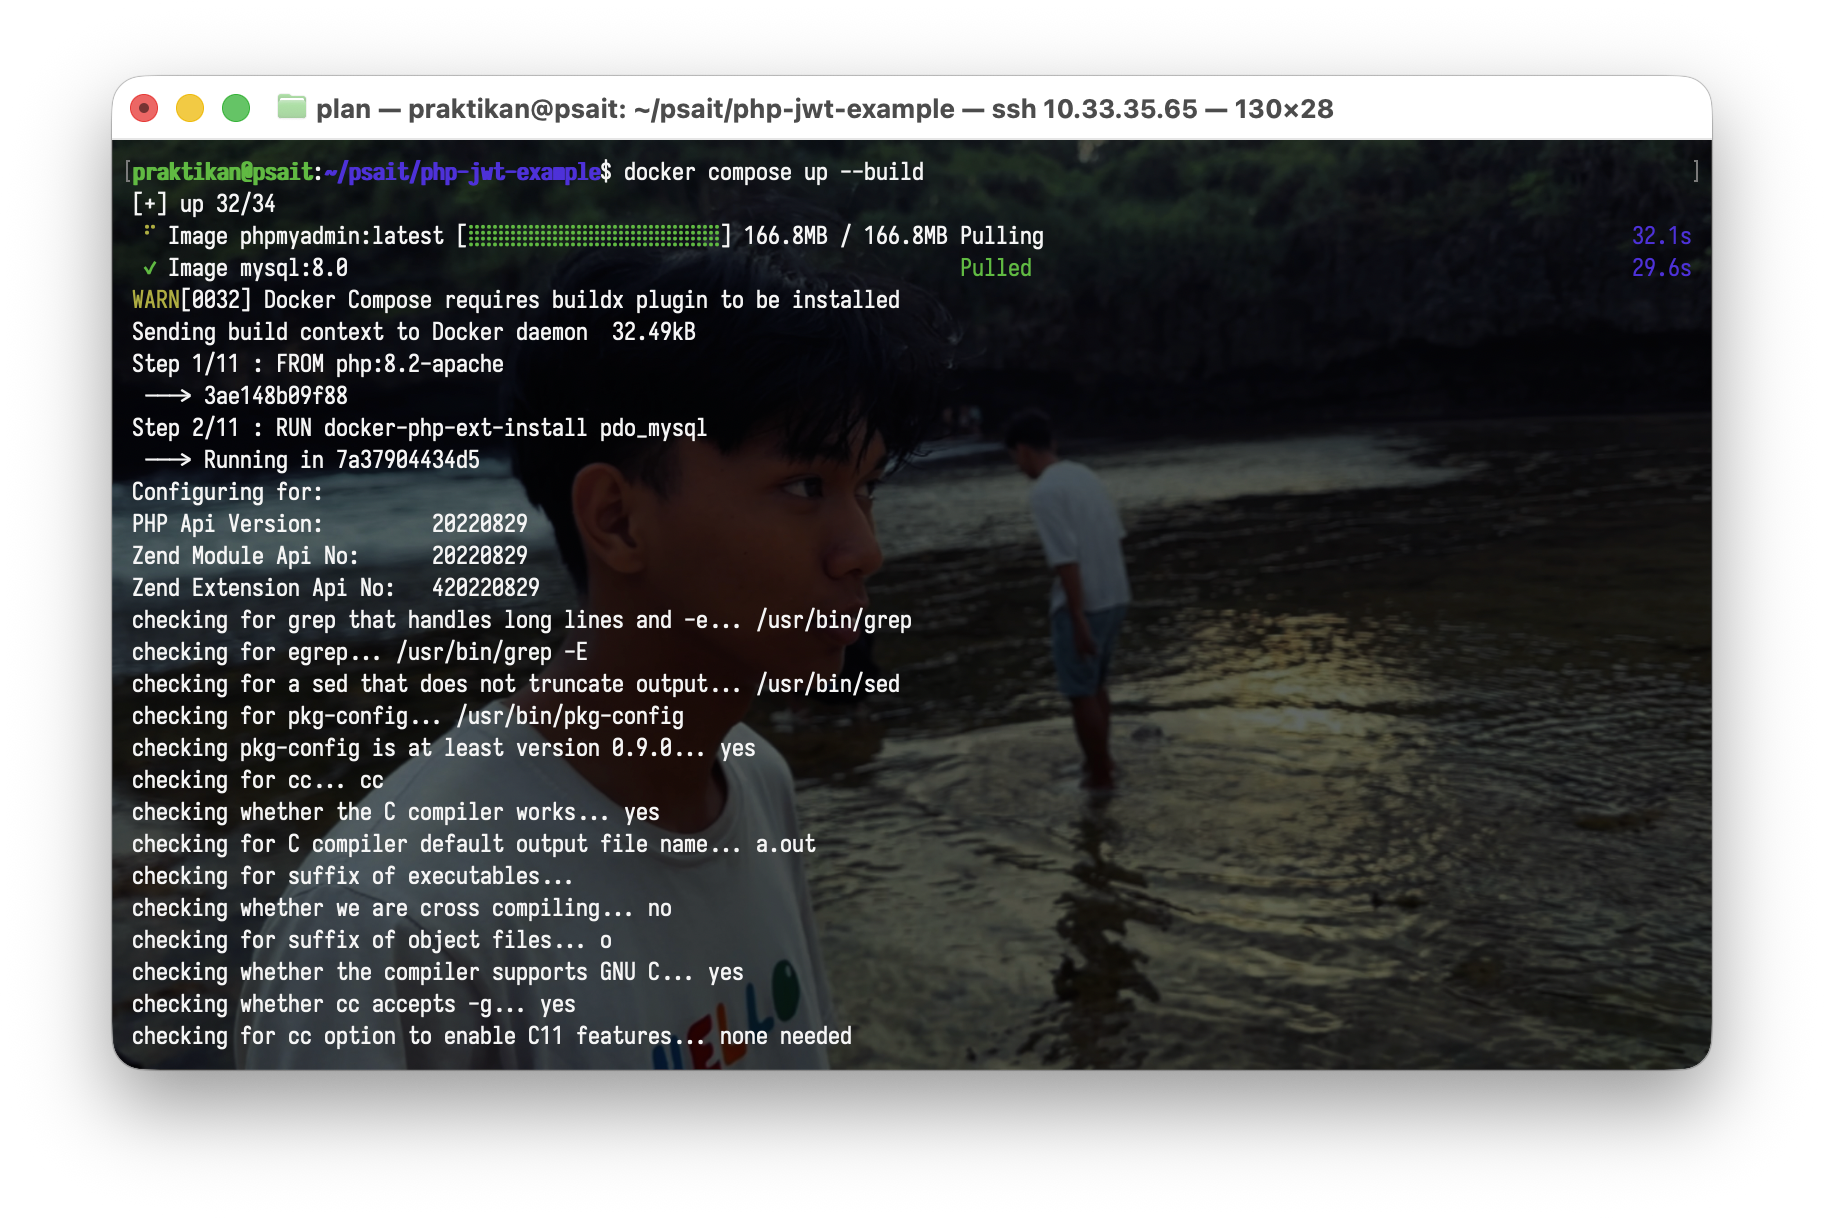
\includegraphics[width=0.85\textwidth]{gambar/04-docker-compose-up-d.png}}
    \caption{Proses Eksekusi docker compose up -d}
    \label{fig:compose_up}
\end{figure}

Kami memverifikasi status operasional seluruh kontainer menggunakan perintah \texttt{docker compose ps} untuk memastikan tidak terjadi crash saat proses inisialisasi awal (Gambar \ref{fig:compose_ps}):
\begin{lstlisting}[style=commonstyle, language=bash]
docker compose ps
\end{lstlisting}
\begin{figure}[H]
    \centering
    \customfbox{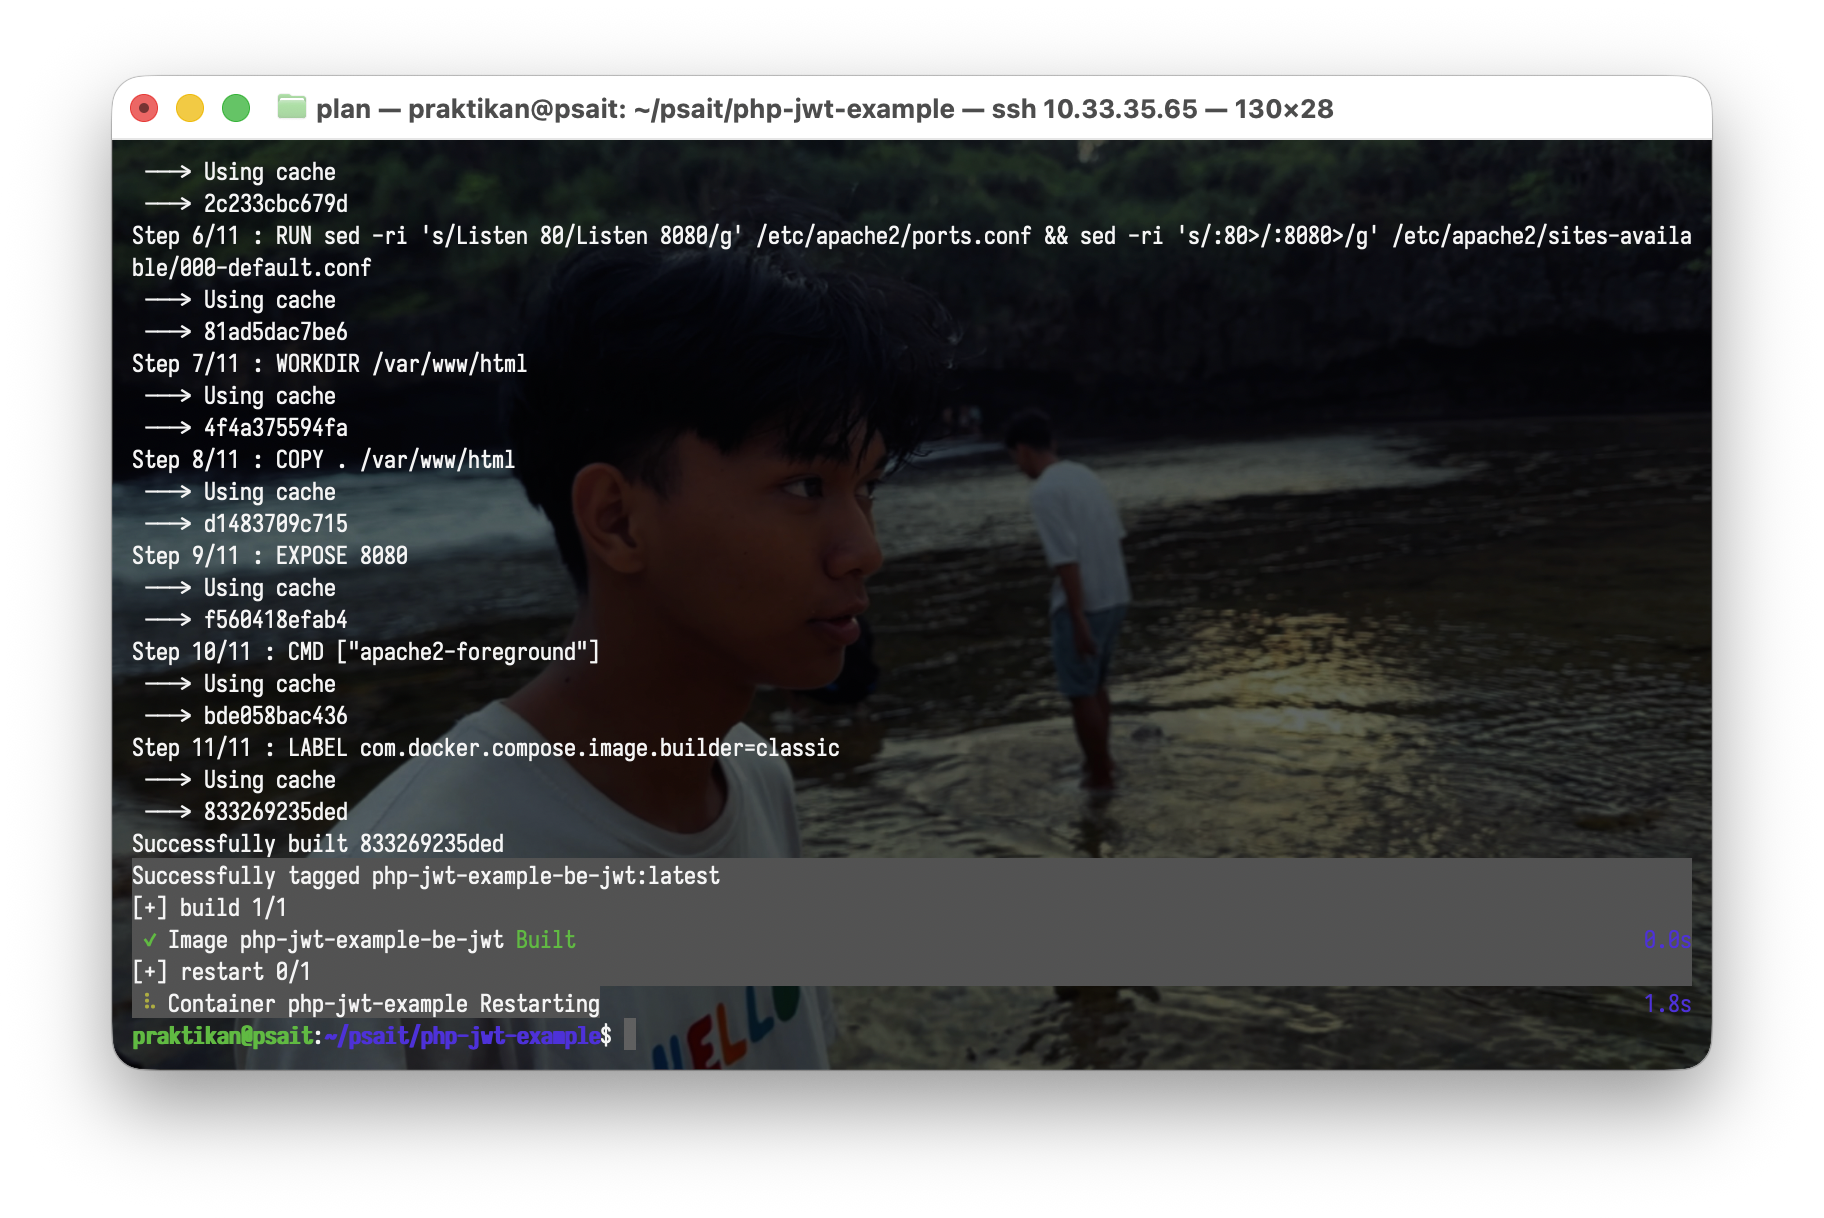
\includegraphics[width=0.85\textwidth]{gambar/05-docker-compose-rebuild-restart.png}}
    \caption{Pengecekan Status Ketiga Kontainer Berstatus Running}
    \label{fig:compose_ps}
\end{figure}

\section{Pembuktian Uji Coba Fitur Hot-Reload}
Untuk membuktikan bahwa mekanisme volume binding berjalan lancar untuk pengembangan program, kami menambahkan endpoint route baru \texttt{/docker} ke dalam \texttt{index.php} menggunakan teks editor lokal secara langsung:
\begin{lstlisting}[style=phpstyle]
    case '/docker':
        http_response_code(200);
        echo json_encode(array("message" => "Docker is working!"));
        break;
\end{lstlisting}
Kami menguji endpoint tersebut secara instan tanpa menghentikan atau membangun ulang kontainer. Perubahan langsung terdeteksi di dalam kontainer dan mengembalikan respons yang sesuai (Gambar \ref{fig:hot_reload}):
\begin{lstlisting}[style=commonstyle, language=bash]
curl -i http://localhost:8080/docker
\end{lstlisting}
\begin{figure}[H]
    \centering
    \customfbox{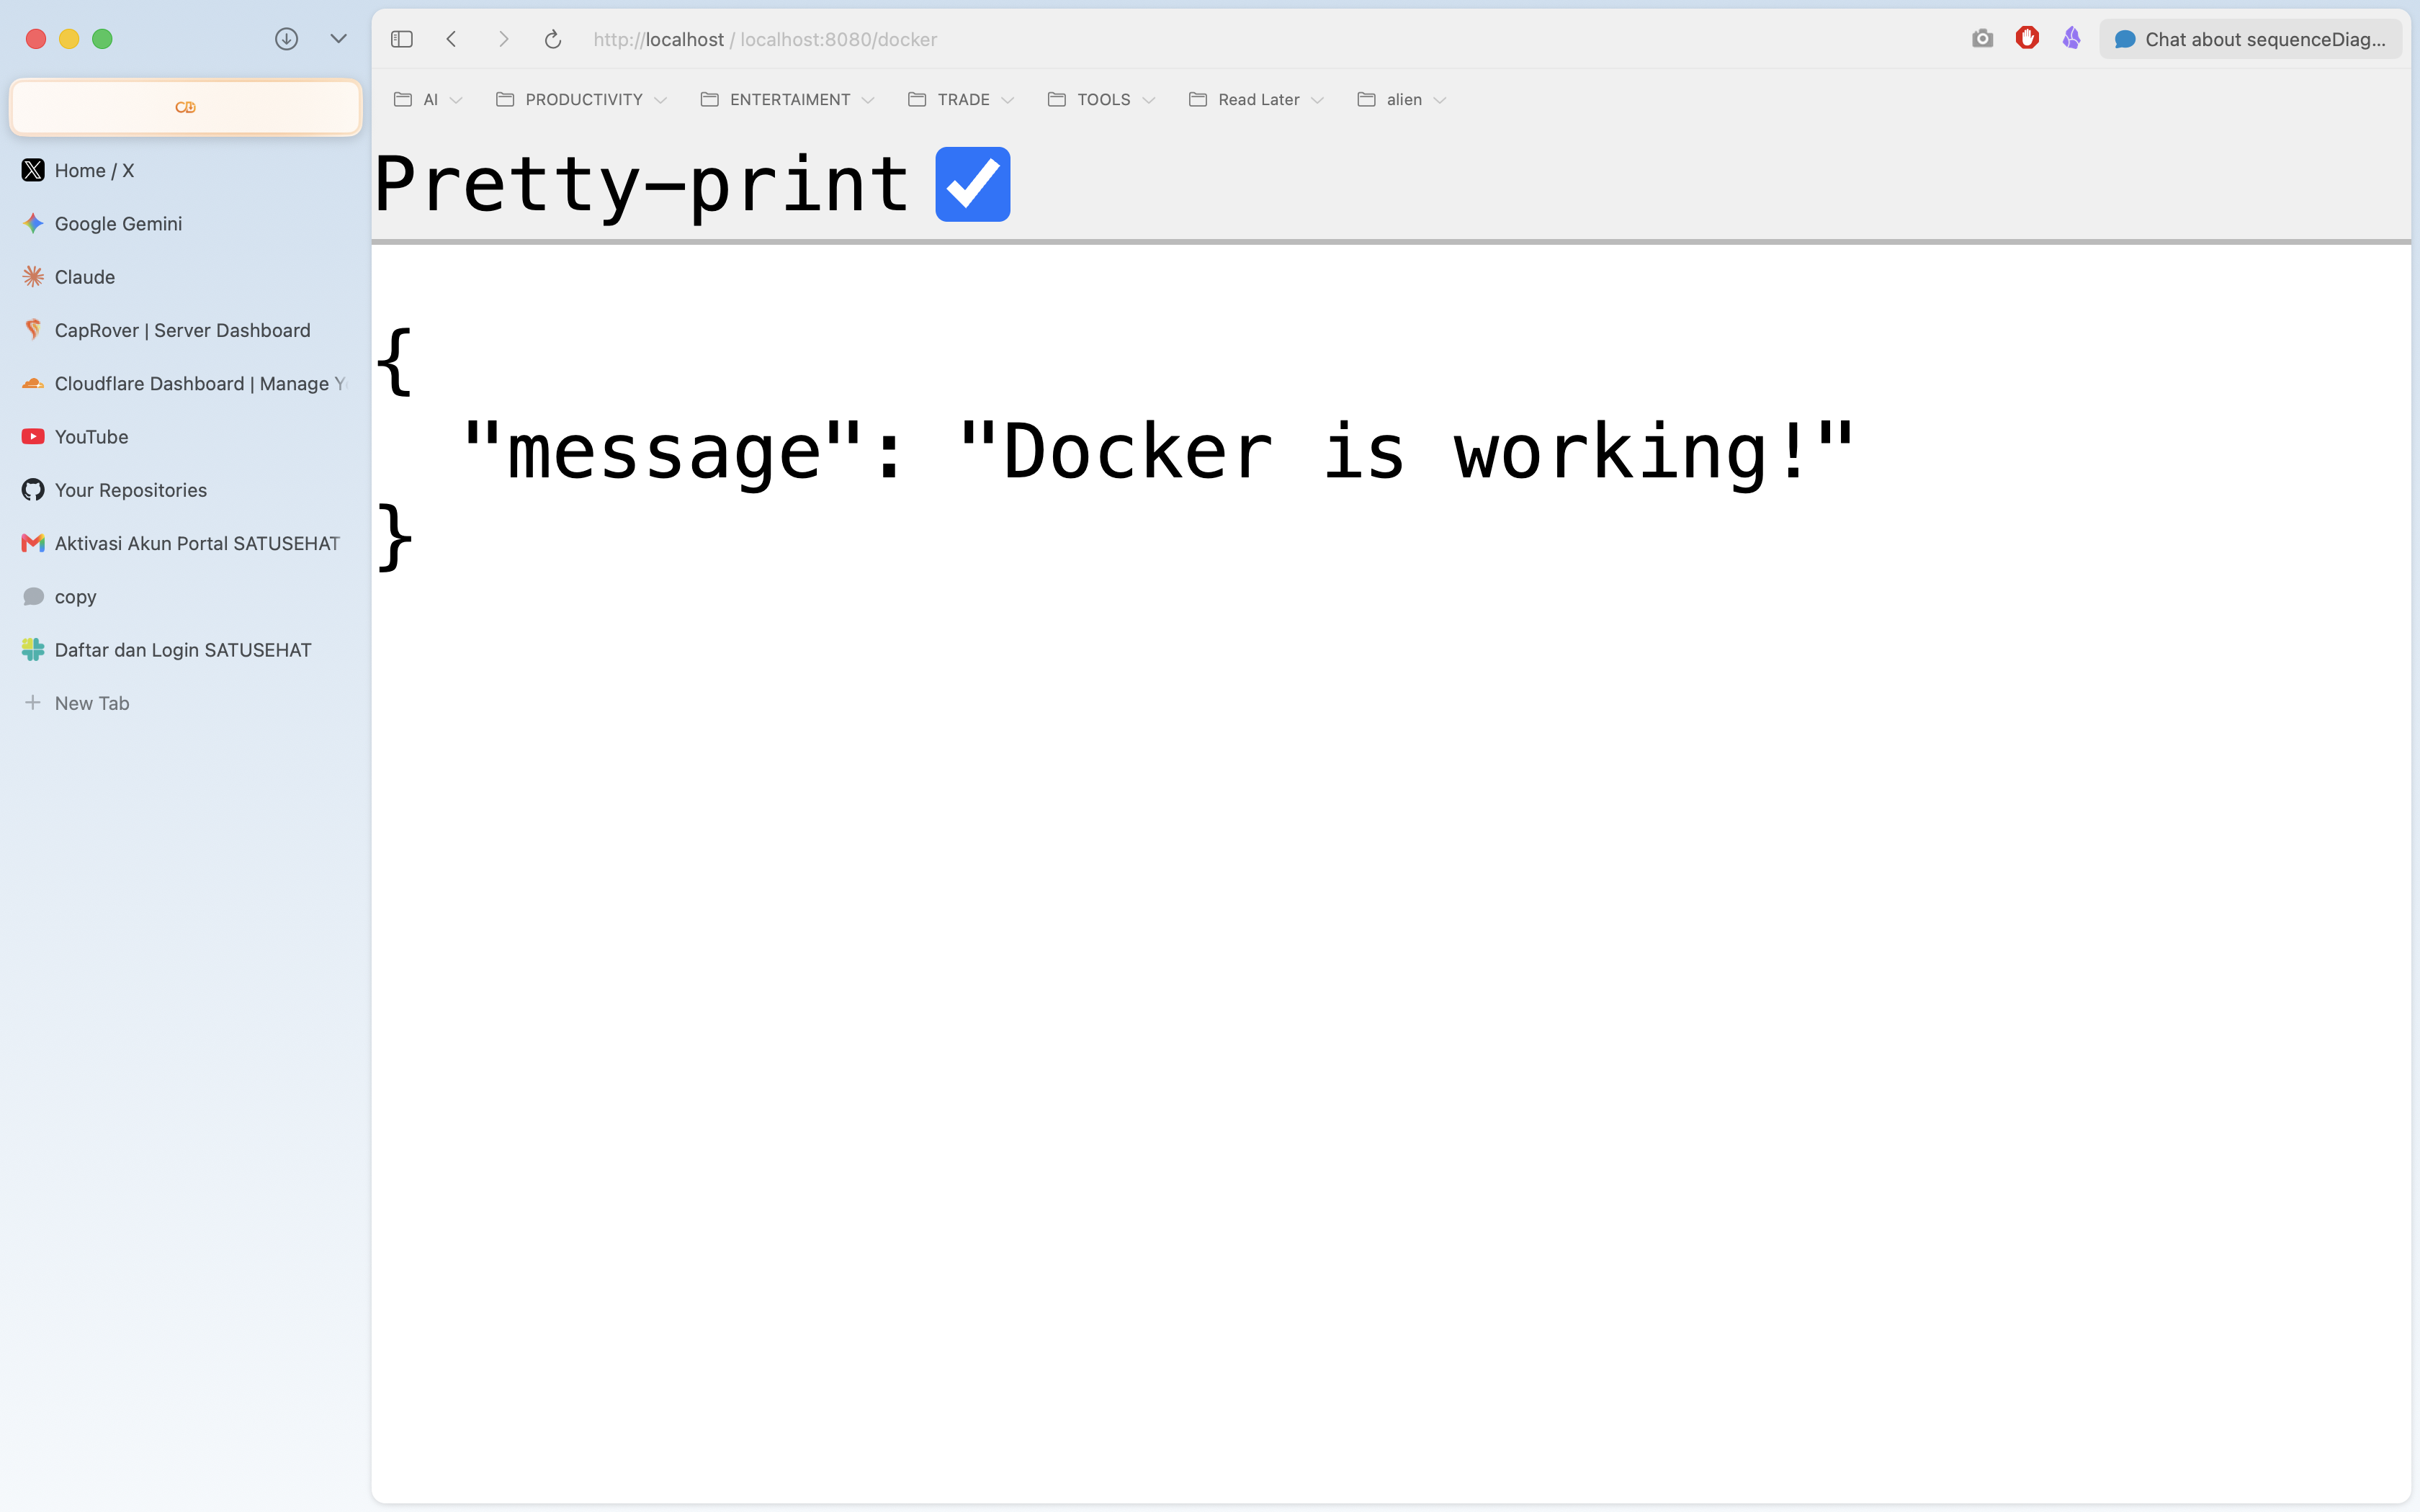
\includegraphics[width=0.85\textwidth]{gambar/16-browser-hot-reload-docker.png}}
    \caption{Output Verifikasi Fungsionalitas Fitur Hot-Reload}
    \label{fig:hot_reload}
\end{figure}

\section{Pengujian REST API Terintegrasi Database}
Dengan basis data MySQL terisolasi yang diorkestrasikan oleh Docker Compose, kami melakukan siklus lengkap pengujian API autentikasi menggunakan Postman:

\subsection{Registrasi Pengguna Baru via API}
Request POST dikirimkan ke endpoint \texttt{http://localhost:8080/api/register} untuk mendaftarkan akun baru dengan peran \texttt{admin} (Gambar \ref{fig:postman_register_compose}).
\begin{figure}[H]
    \centering
    \customfbox{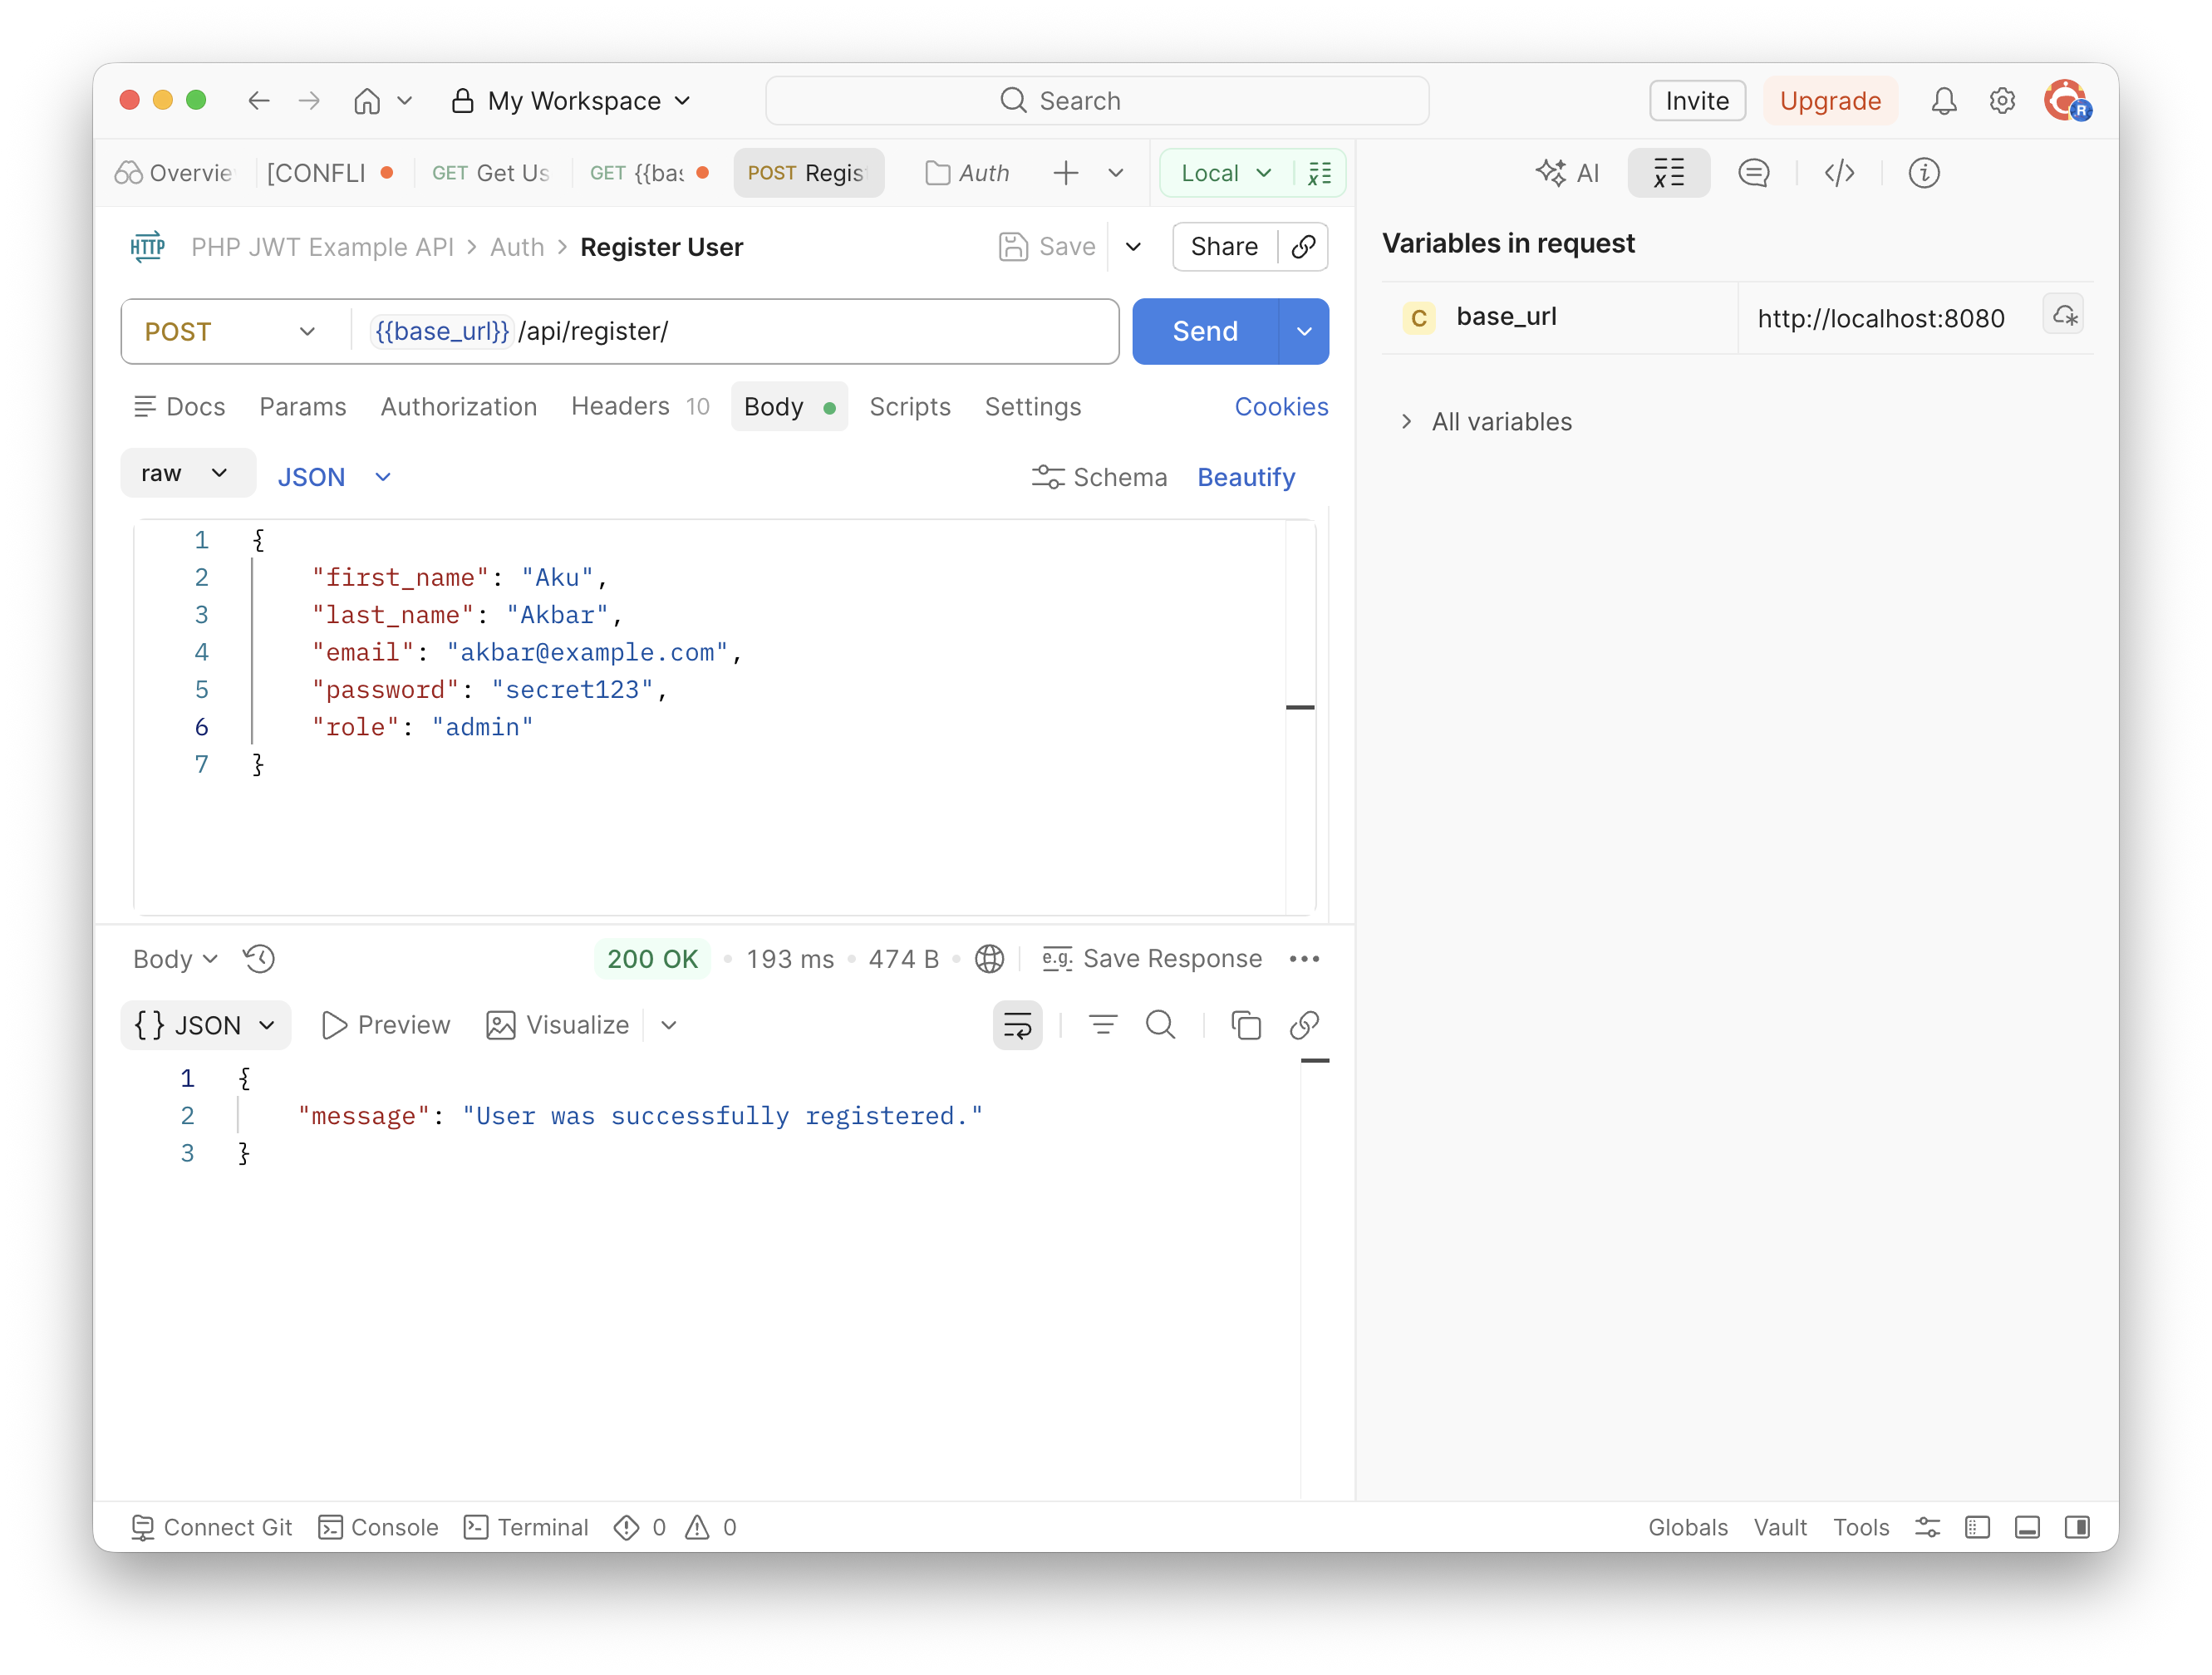
\includegraphics[width=0.85\textwidth]{gambar/12-postman-api-register.png}}
    \caption{Registrasi Pengguna Baru Sukses Melalui Kontainer API}
    \label{fig:postman_register_compose}
\end{figure}

\subsection{Autentikasi Login dan Generate JWT}
Kredensial akun yang didaftarkan dikirimkan ke endpoint \texttt{/api/login} untuk memicu pembuatan JSON Web Token (JWT) terenkripsi di server (Gambar \ref{fig:postman_login_compose}).
\begin{figure}[H]
    \centering
    \customfbox{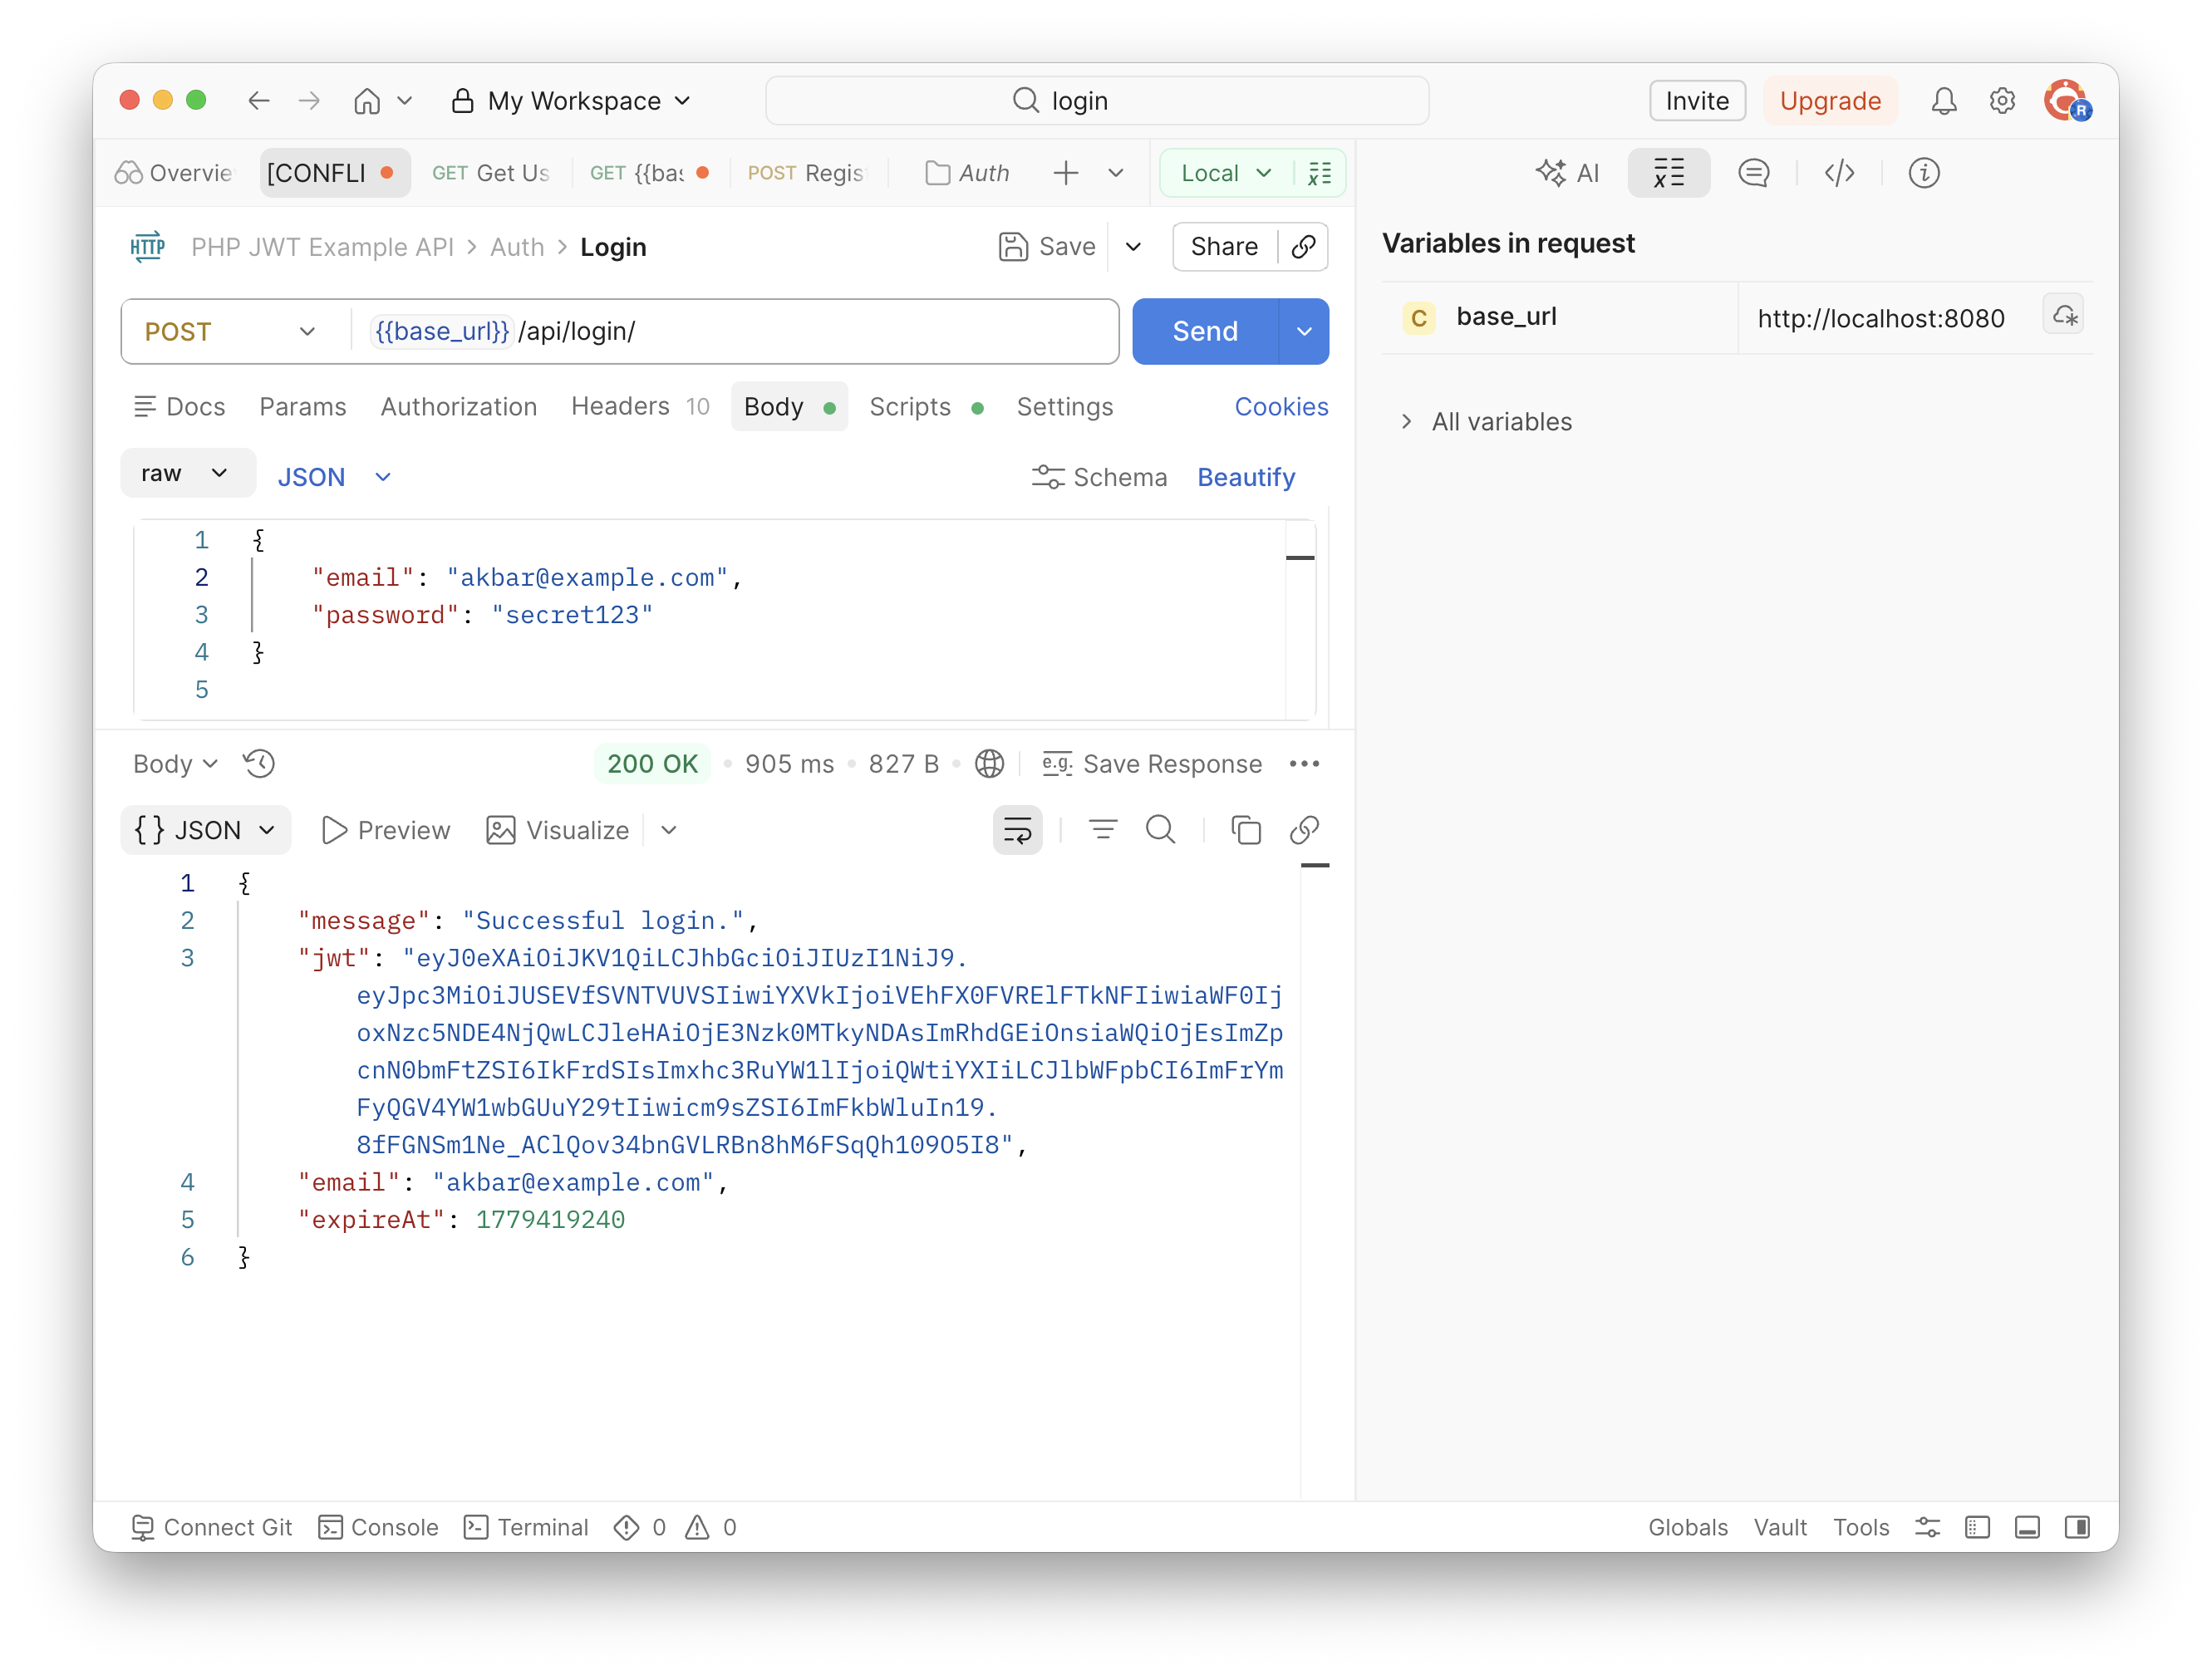
\includegraphics[width=0.85\textwidth]{gambar/13-postman-api-login.png}}
    \caption{Autentikasi Berhasil Menghasilkan Token JWT}
    \label{fig:postman_login_compose}
\end{figure}

\subsection{Akses Halaman Terproteksi dengan Bearer Token}
Token JWT yang dihasilkan disematkan di dalam request header Authorization Bearer untuk mengakses endpoint data pengguna \texttt{/api/users}. Kontainer API PHP mendekodekan token tersebut dan berhasil mengizinkan akses karena peran user divalidasi sebagai administrator (Gambar \ref{fig:postman_users_compose}).
\begin{figure}[H]
    \centering
    \customfbox{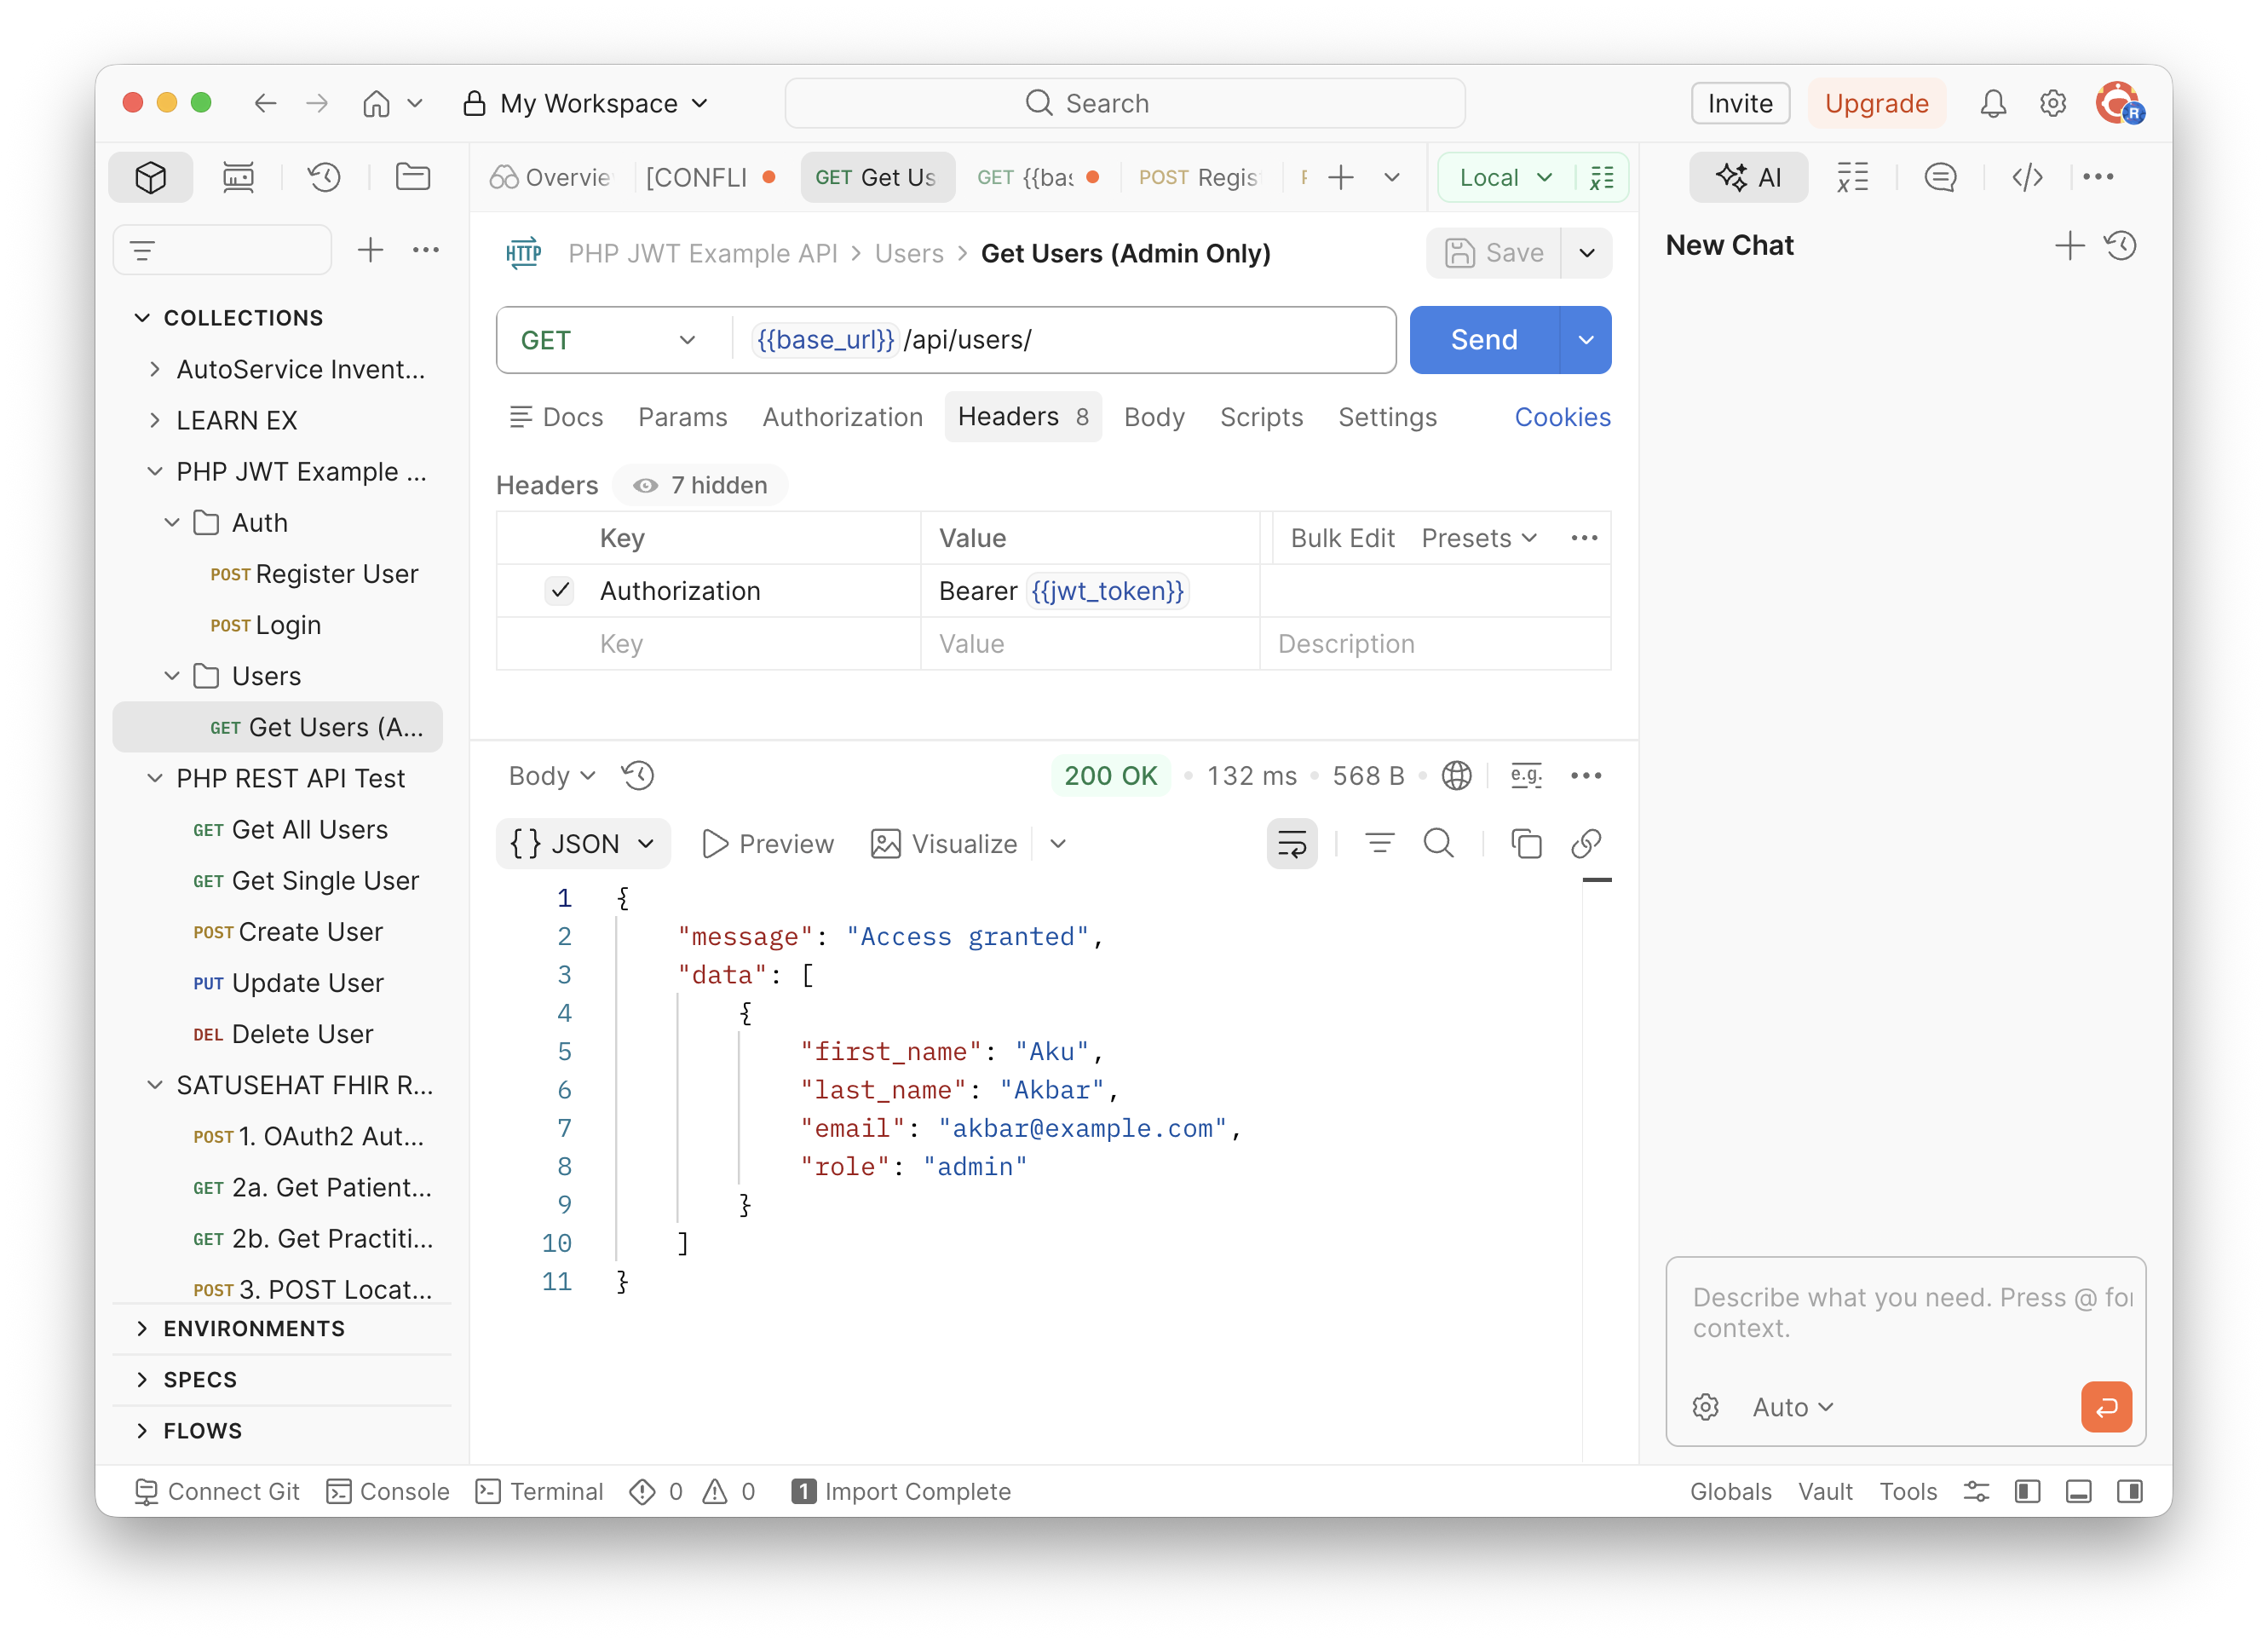
\includegraphics[width=0.85\textwidth]{gambar/14-postman-api-get-users.png}}
    \caption{Pengaksesan Halaman Terproteksi dengan Validasi JWT}
    \label{fig:postman_users_compose}
\end{figure}

\section{Tugas dan Analisis Tambahan}

\subsection{Integrasi Service phpMyAdmin}
Untuk mempermudah manajemen database tanpa terminal, kami berhasil memuat layanan phpMyAdmin ke dalam konfigurasi orkestrasi di port \texttt{8081}. Verifikasi koneksi membuktikan phpMyAdmin berhasil terhubung ke basis data kontainer \texttt{database\_mysql} melalui jaringan virtual Docker host (Gambar \ref{fig:pma_web}):
\begin{lstlisting}[style=commonstyle, language=bash]
curl -i http://localhost:8081
\end{lstlisting}
\begin{figure}[H]
    \centering
    \customfbox{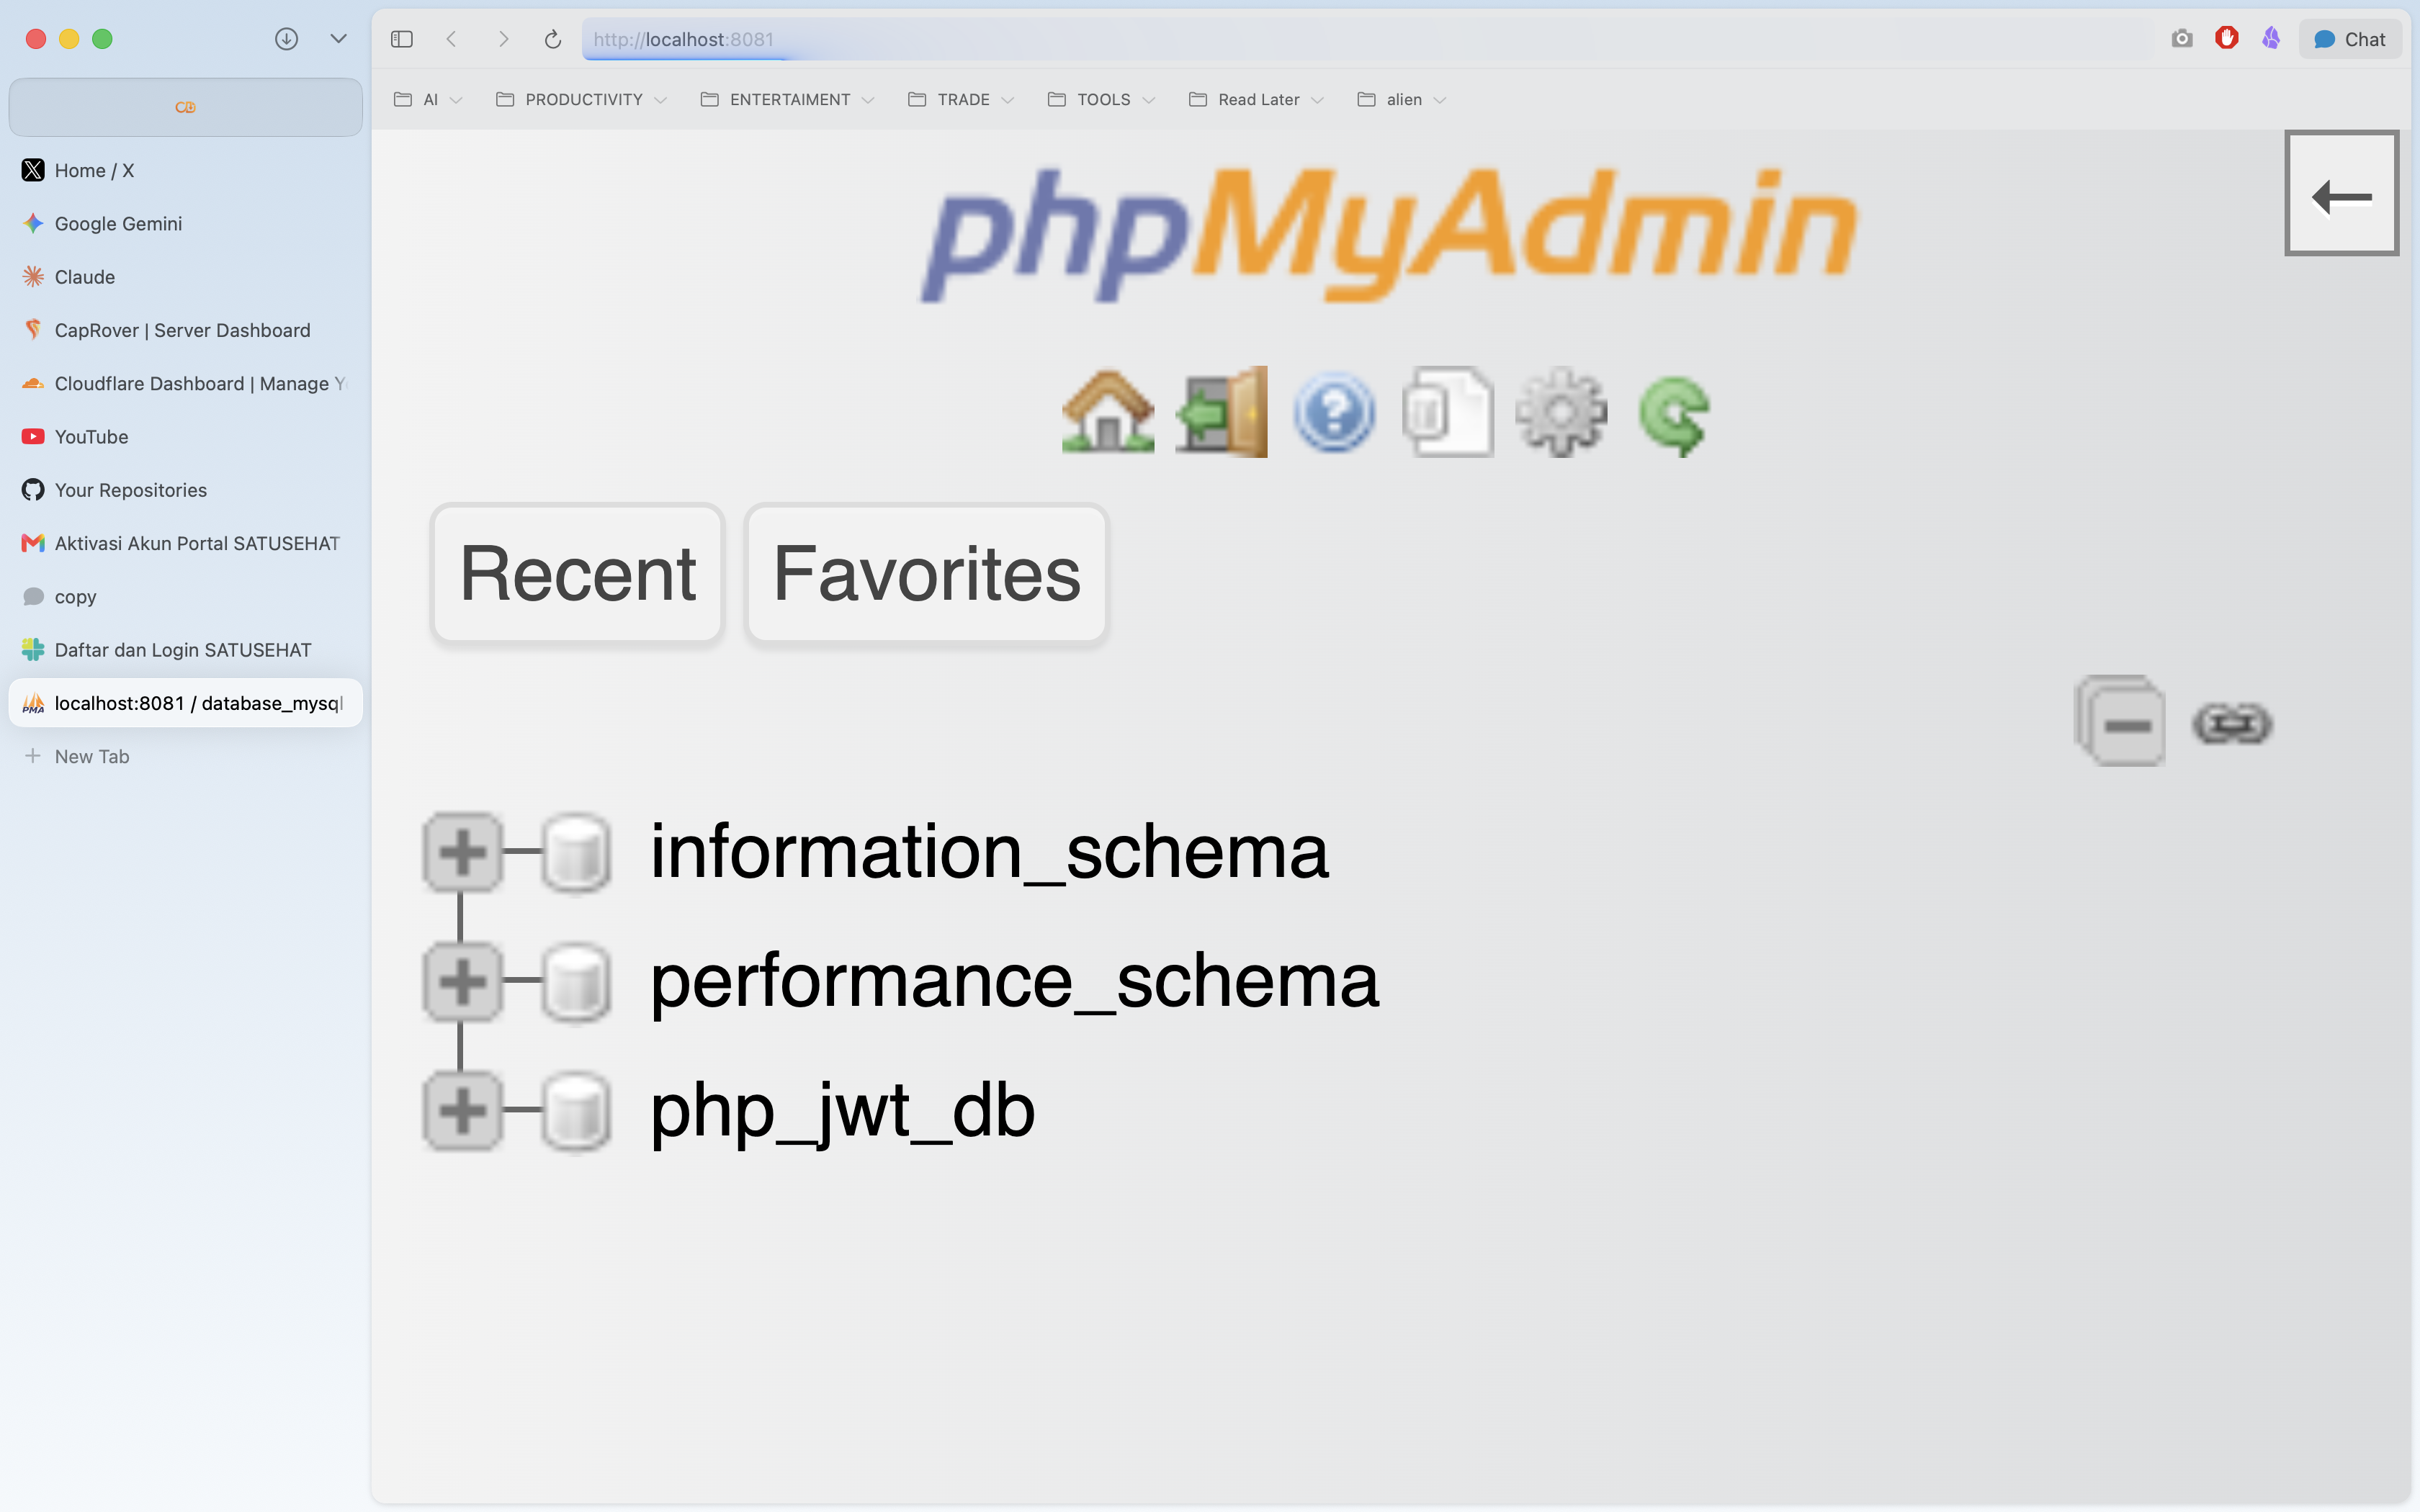
\includegraphics[width=0.85\textwidth]{gambar/17-phpmyadmin-web.png}}
    \caption{Tampilan phpMyAdmin yang Terkoneksi ke Database Kontainer}
    \label{fig:pma_web}
\end{figure}

\subsection{Pengecekan dan Verifikasi CRUD Basis Data}
Untuk memverifikasi integrasi penuh basis data yang diorkestrasikan oleh Docker Compose dan diakses secara visual menggunakan phpMyAdmin, kami menjalankan serangkaian pengujian manipulasi data CRUD (Create, Read, Update, Delete) pada tabel \texttt{users} secara visual melalui GUI phpMyAdmin:
\begin{enumerate}
    \item \textbf{CREATE}: Menguji registrasi API berhasil menambahkan baris data baru ke dalam database secara otomatis.
    
    \item \textbf{READ}: Membaca dan memverifikasi baris data baru yang telah tersimpan sempurna di tabel \texttt{users} secara visual melalui antarmuka GUI phpMyAdmin (Gambar \ref{fig:pma_read}).
    \begin{figure}[H]
        \centering
        \customfbox{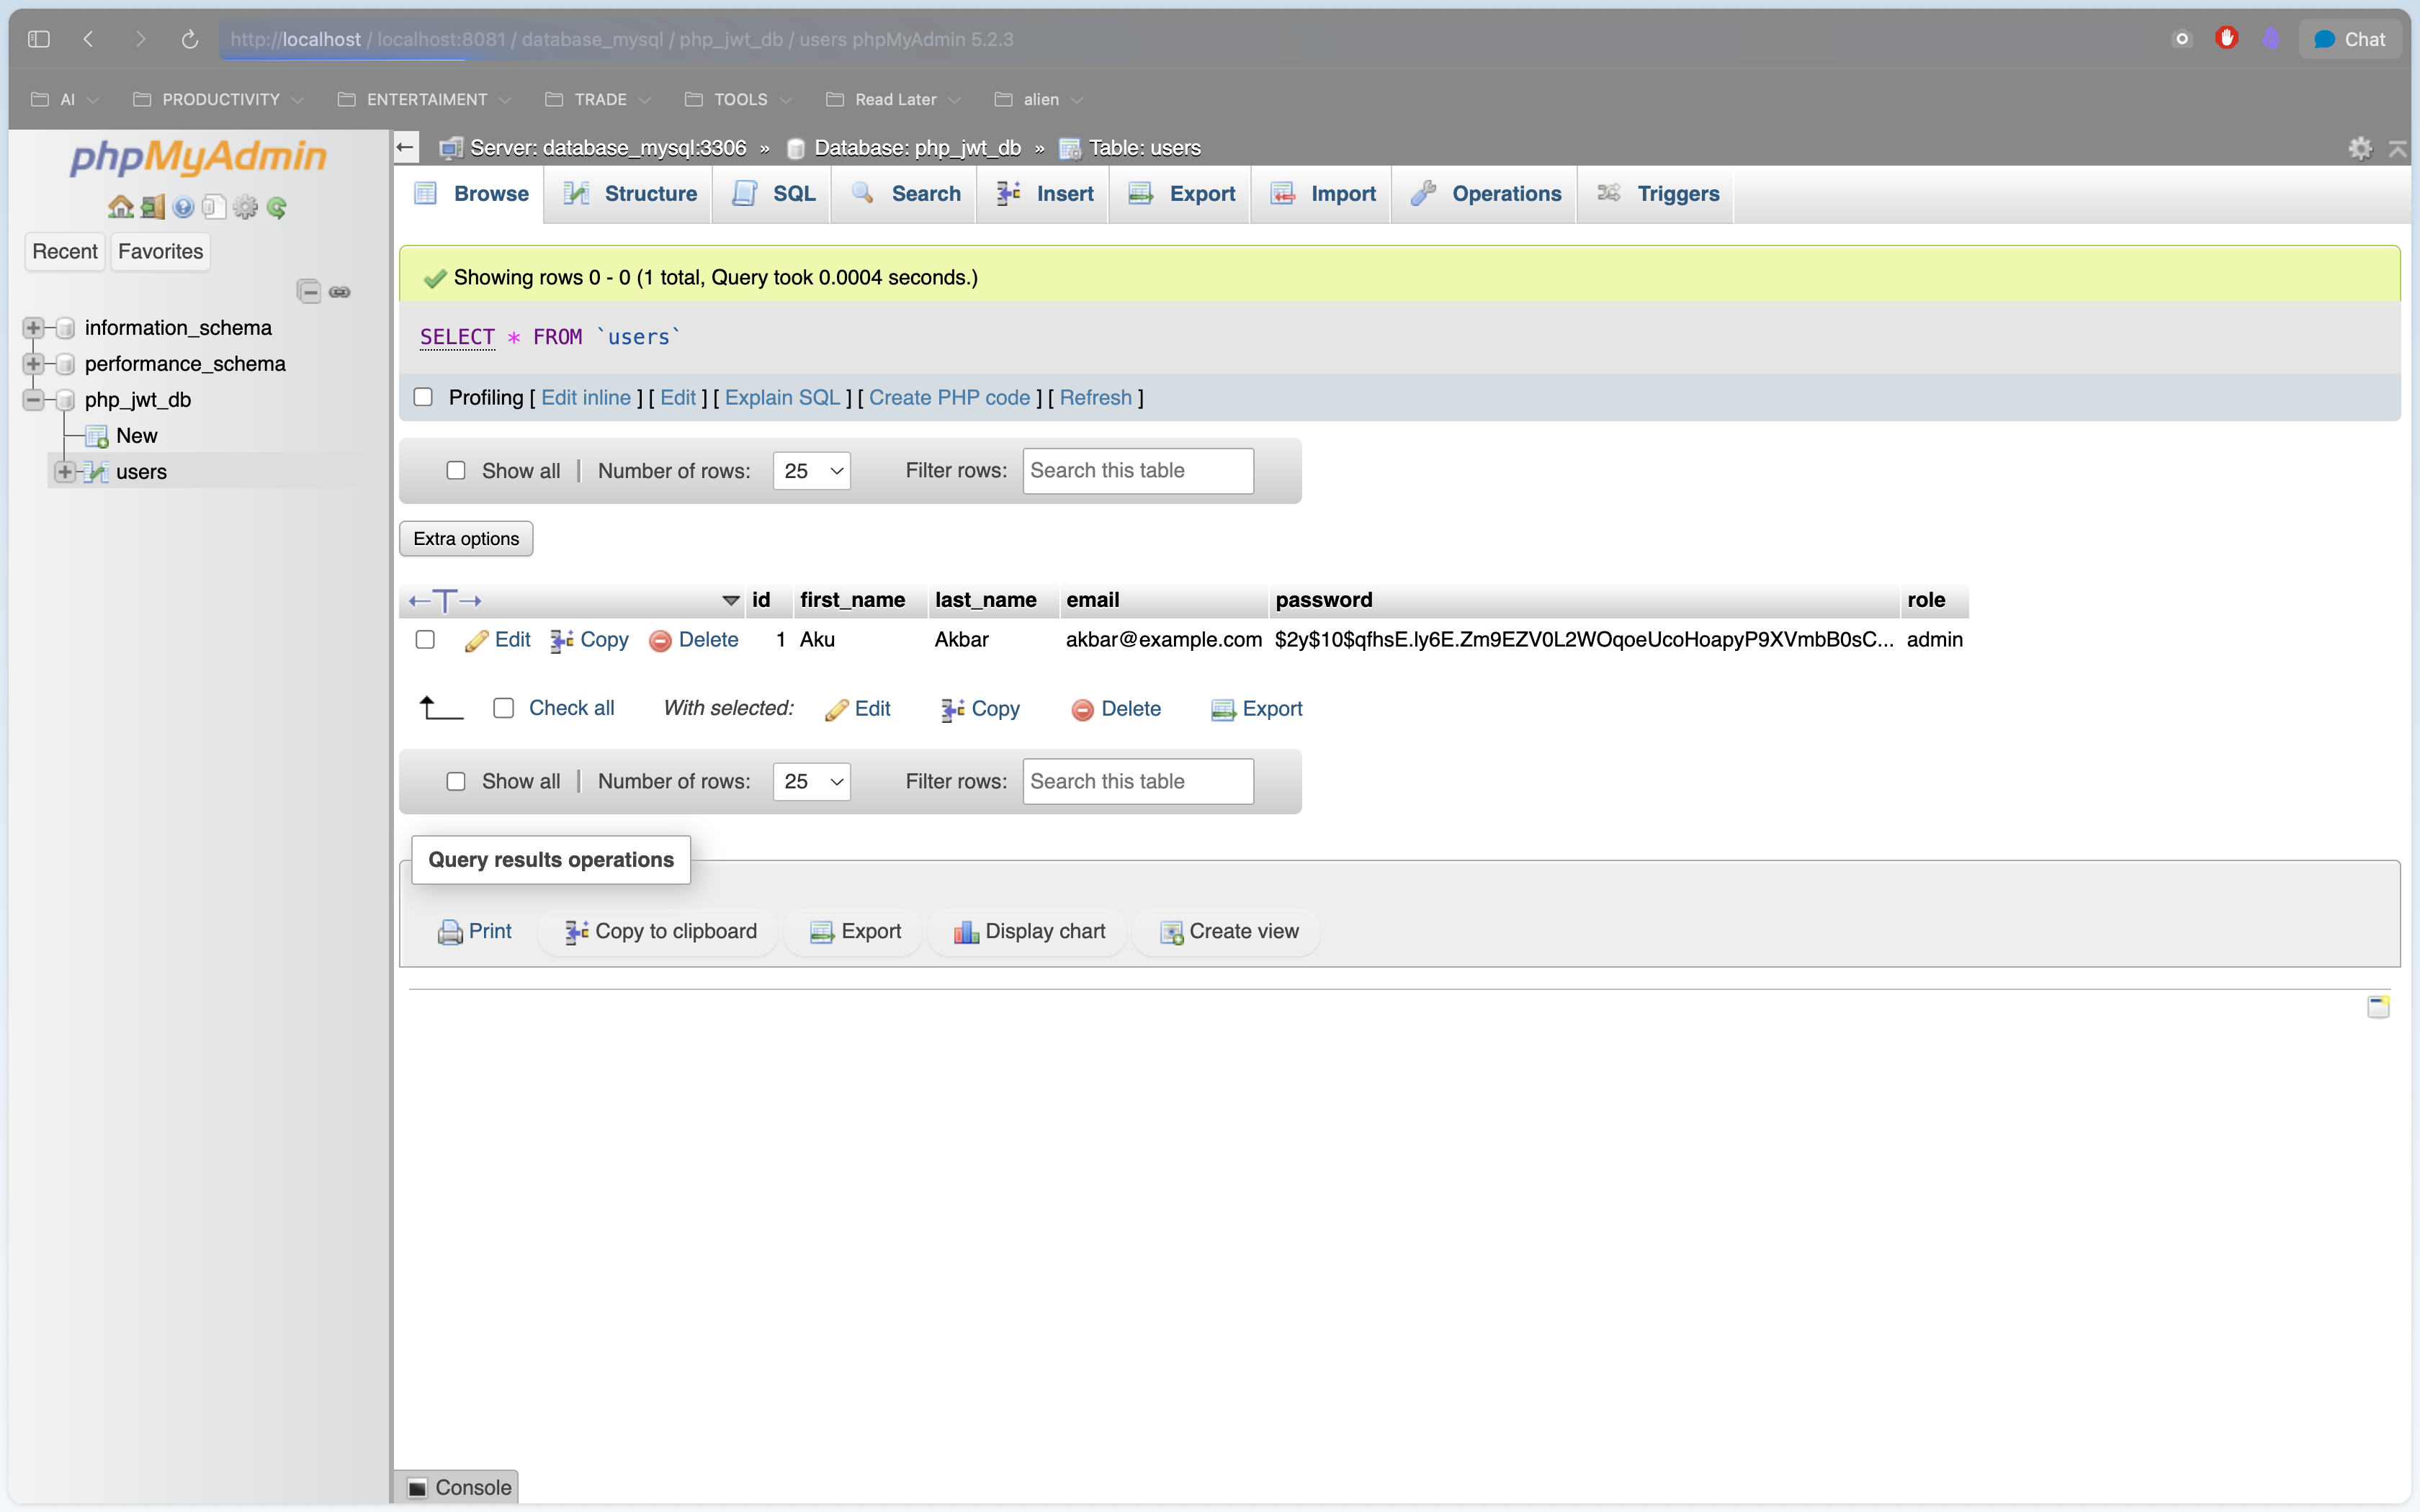
\includegraphics[width=0.85\textwidth]{gambar/18-phpmyadmin-crud-read.png}}
        \caption{Verifikasi Data Hasil Registrasi Sukses Melalui GUI phpMyAdmin (READ)}
        \label{fig:pma_read}
    \end{figure}

    \item \textbf{UPDATE}: Melakukan pembaruan (*update*) data pada kolom \texttt{last\_name} secara langsung melalui fitur edit GUI di phpMyAdmin (Gambar \ref{fig:pma_update}).
    \begin{figure}[H]
        \centering
        \customfbox{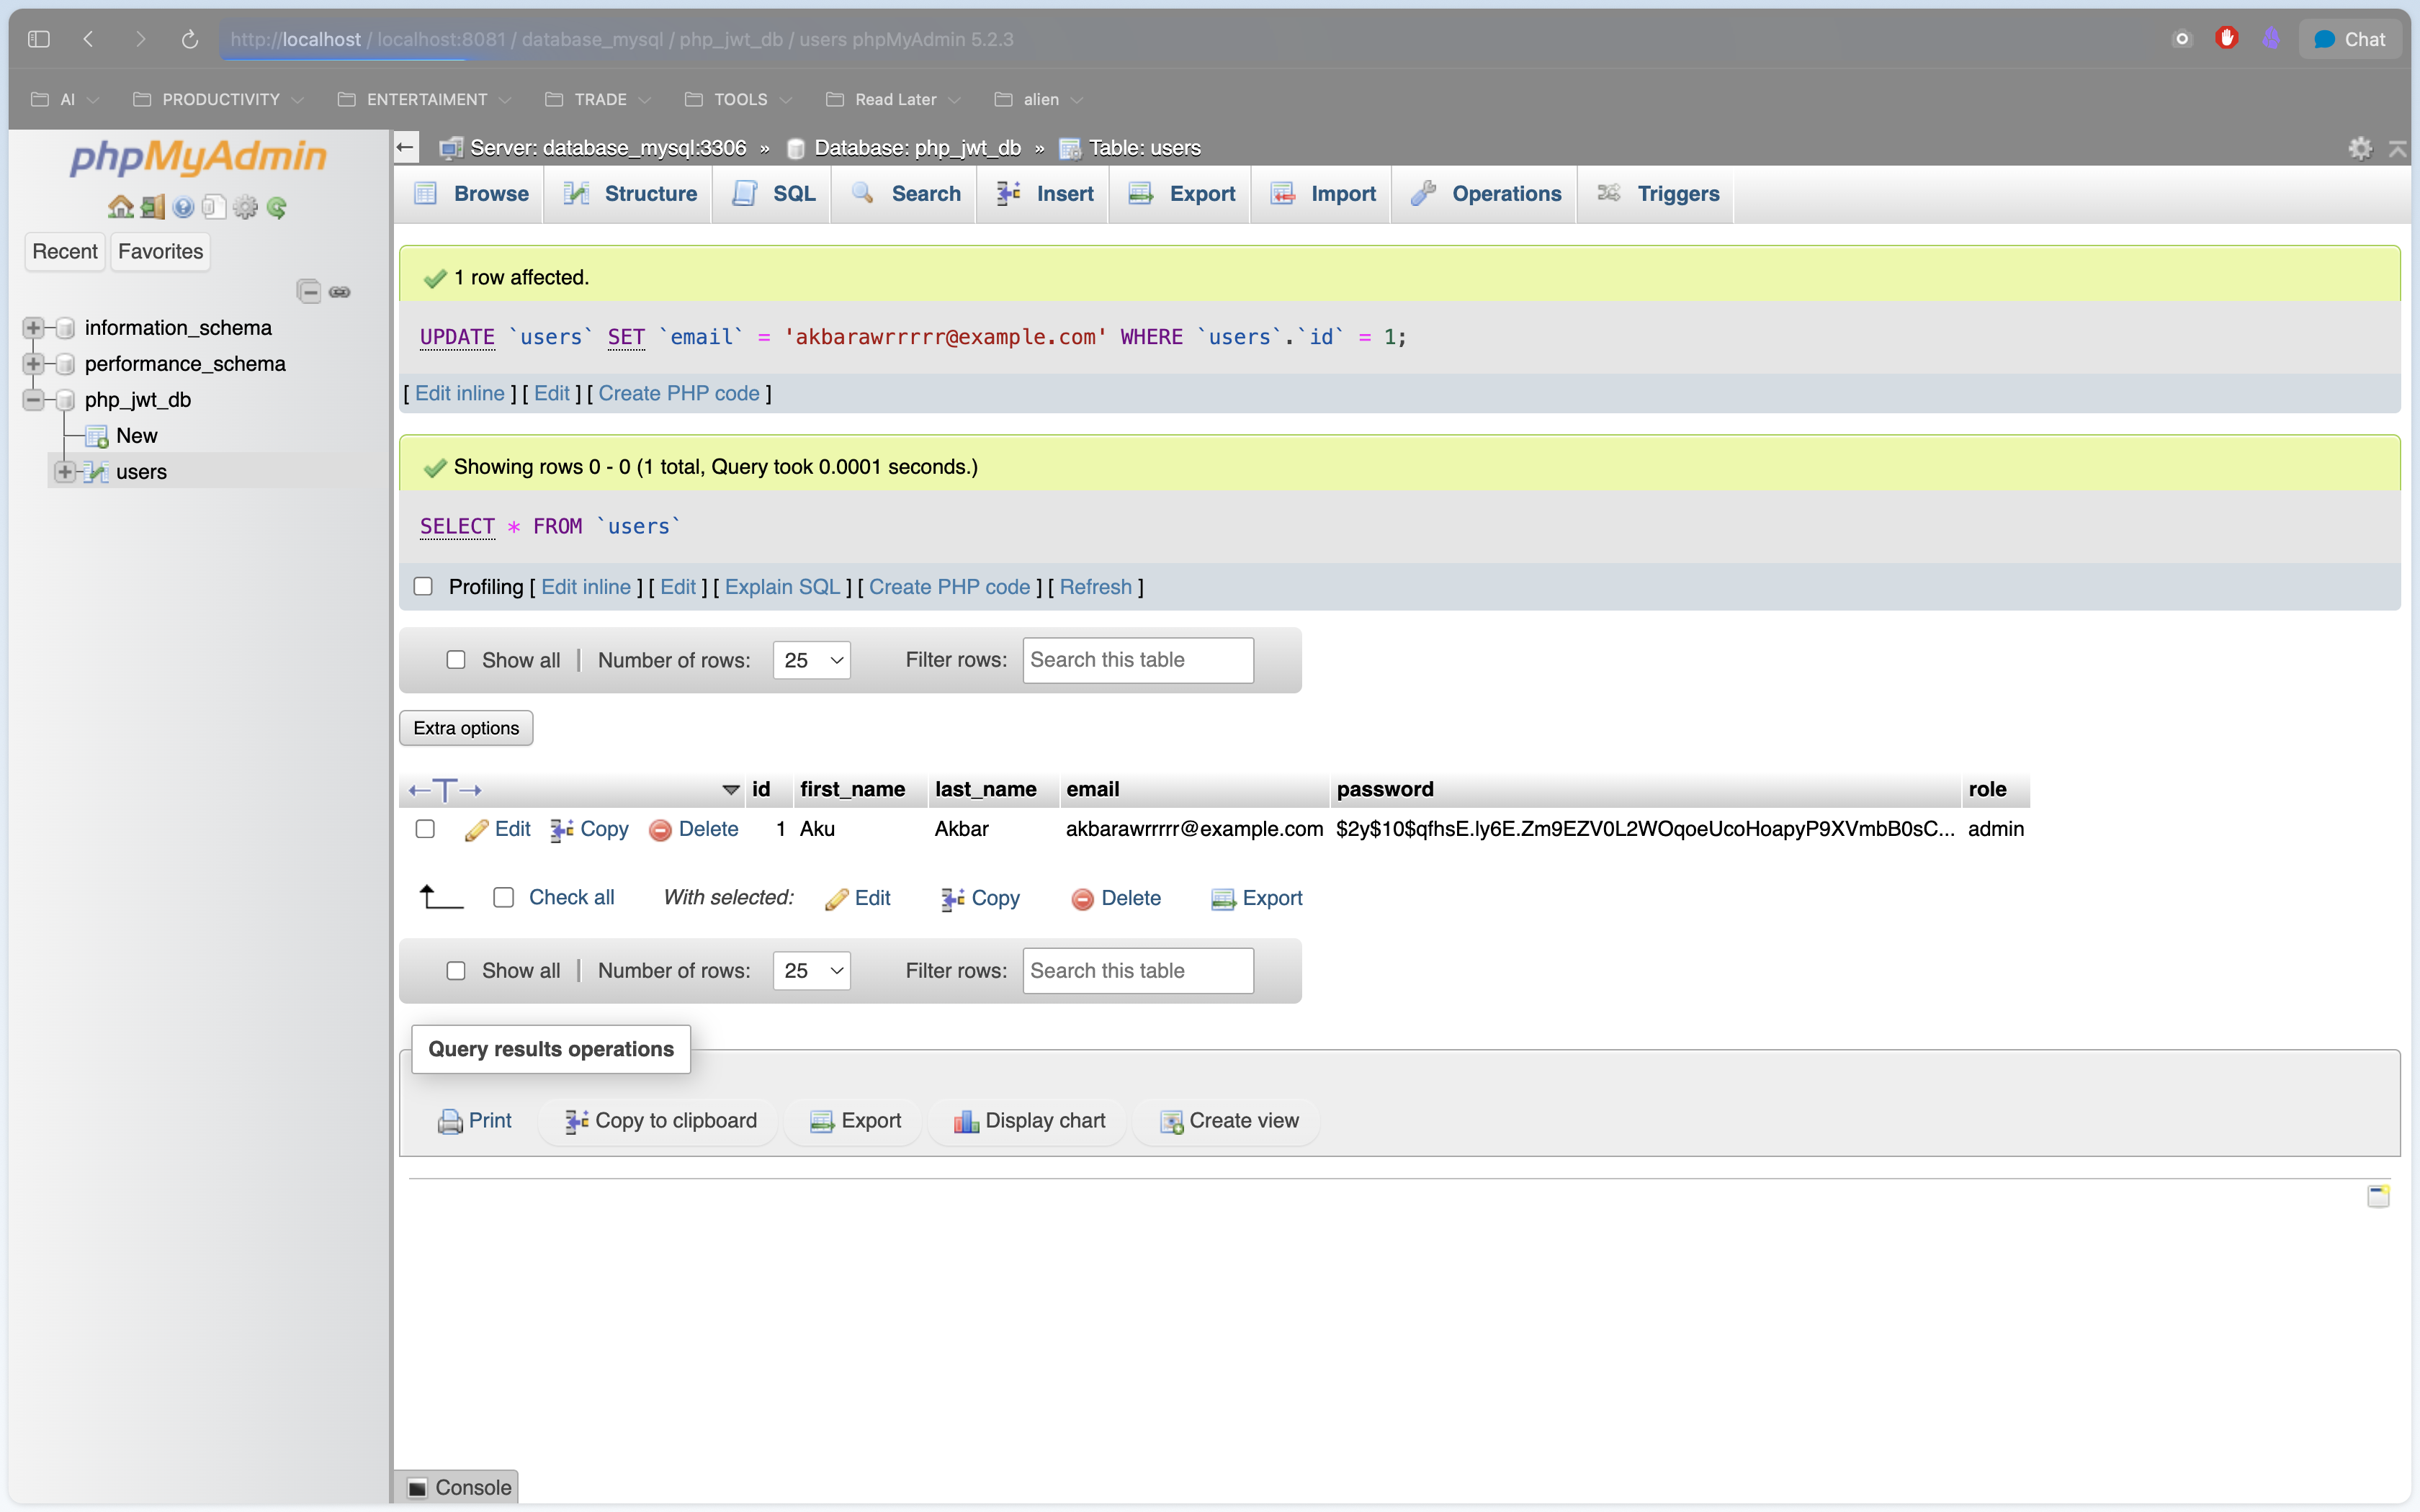
\includegraphics[width=0.85\textwidth]{gambar/19-phpmyadmin-crud-update.png}}
        \caption{Proses Pembaruan Data Pengguna Menggunakan GUI phpMyAdmin (UPDATE)}
        \label{fig:pma_update}
    \end{figure}

    \item \textbf{DELETE}: Melakukan penghapusan (*delete*) baris data pengguna dari tabel \texttt{users} menggunakan tombol hapus pada GUI phpMyAdmin untuk memverifikasi integritas basis data (Gambar \ref{fig:pma_delete}).
    \begin{figure}[H]
        \centering
        \customfbox{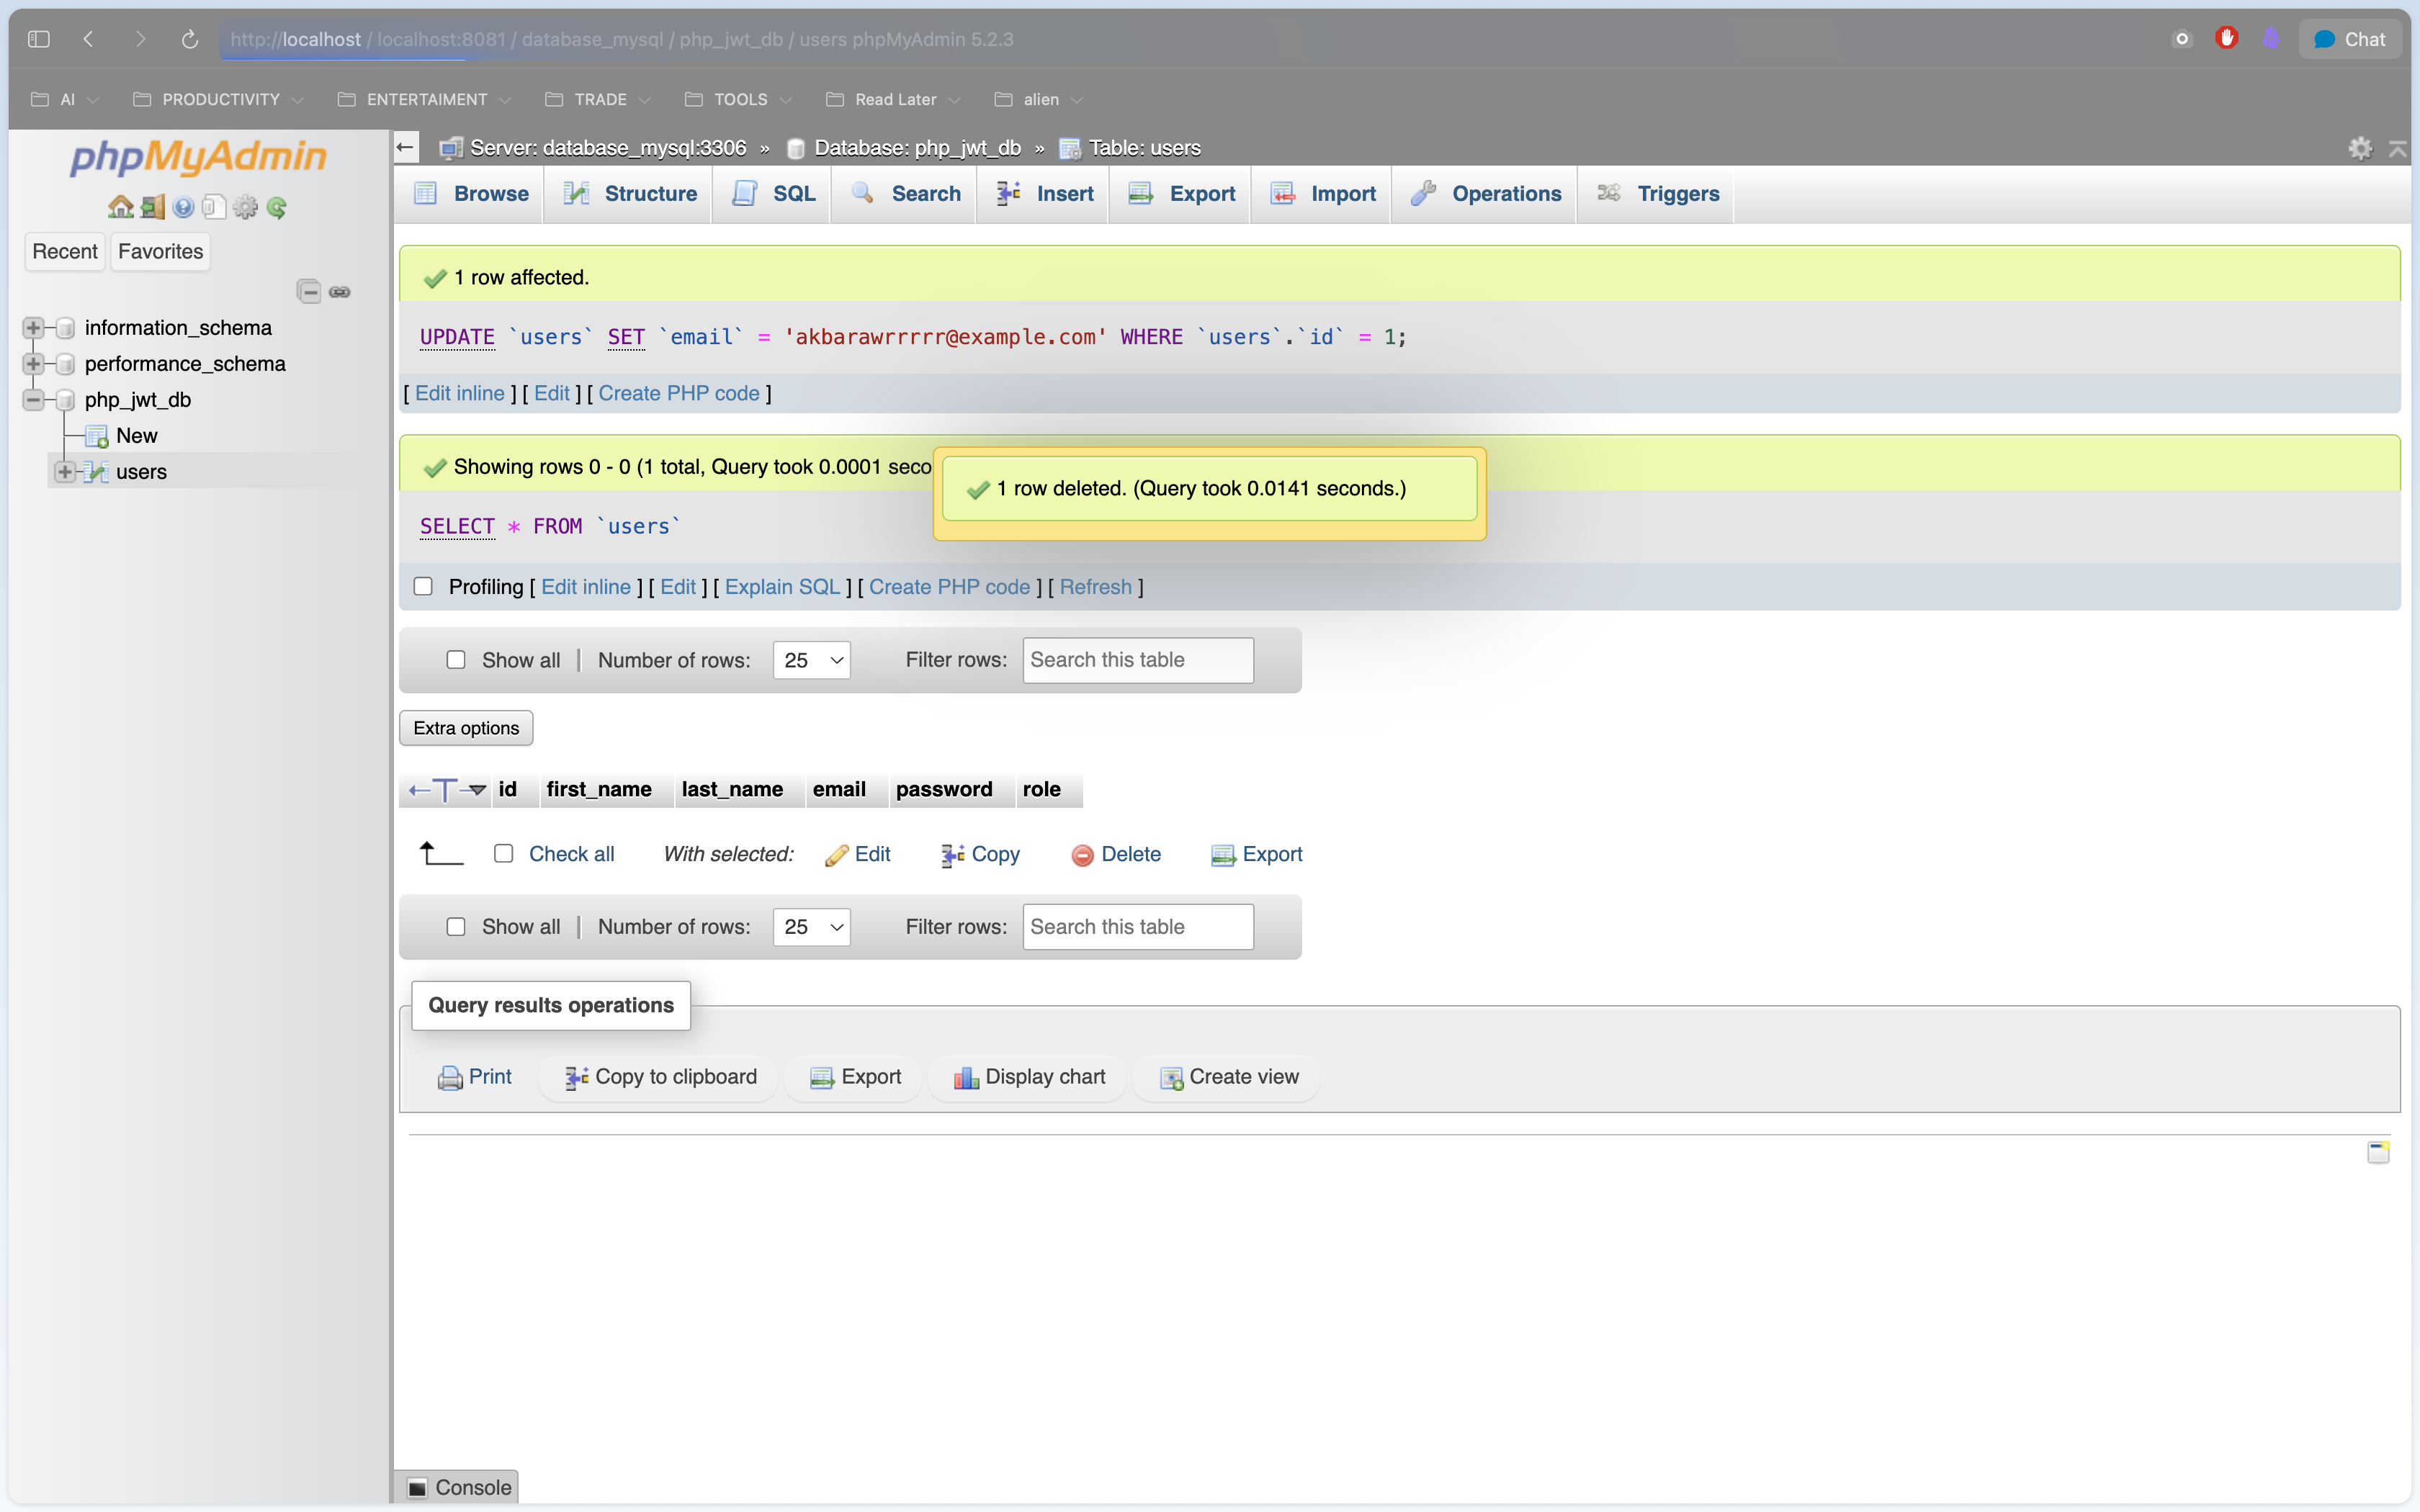
\includegraphics[width=0.85\textwidth]{gambar/20-phpmyadmin-crud-delete.png}}
        \caption{Penghapusan Baris Data Pengguna Berhasil Dilakukan via GUI phpMyAdmin (DELETE)}
        \label{fig:pma_delete}
    \end{figure}
\end{enumerate}
Pembuktian visual ini menegaskan bahwa integritas data, persistensi volume, dan sistem jaringan terdistribusi Docker Compose berfungsi 100\% tanpa hambatan.

\clearpage

\chapter{Kesimpulan}
Praktikum ini berhasil membuktikan keandalan dan kemudahan yang ditawarkan oleh Docker Compose dalam mengelola arsitektur aplikasi multi-kontainer. Melalui definisi berkas konfigurasi \texttt{docker-compose.yml}, kita dapat dengan mudah menyatukan komponen web server PHP-Apache, basis data MySQL 8.0, dan alat administrasi phpMyAdmin ke dalam satu orkestrasi jaringan virtual bridge yang terisolasi dan aman. 

Fitur **Volume Binding** mempercepat proses pengembangan melalui hot-reload instan tanpa perlu rebuild image berulang kali, sementara **Persistent Volume** memberikan jaminan keamanan data basis data. Kesimpulannya, Docker Compose menyederhanakan siklus DevOps dan deployment aplikasi terdistribusi secara signifikan.

\clearpage
\addcontentsline{toc}{chapter}{Daftar Pustaka}
\renewcommand{\bibname}{Daftar Pustaka}
\begin{thebibliography}{99}
    \bibitem{docker_docs} Docker, \textit{Docker Compose Documentation}. [Online]. Tersedia: \url{https://docs.docker.com/compose/}.
\end{thebibliography}

\end{document}
